\documentclass{article}
\usepackage{graphicx}
\graphicspath{{recursos/}}

% cor das caixas
\usepackage{xcolor}
\definecolor{azul}{RGB}{39,90,192}

% pacote de configuração
\usepackage[
    nome = SciDavis,
    cor  = azul,
    logo = logo.pdf
]{pacotes/tutorial}

% pacotes extras
\usepackage{caption, subcaption, pdfpages, wrapfig}
\usepackage{circuitikz, graphics, float}

% começa a seção no `0`
\setcounter{section}{-1}



\hypersetup{
    pdftitle  = {Gráficos no SciDavis},
    pdfauthor = {Tiago de Paula}
}

\title{Criação e Formatação de Gráficos com o}\softwarelogo
\author{\href{mailto:t187679@dac.unicamp.br}{Tiago de Paula}}
\date{}


\begin{document}
    \maketitle

    Na começo dos anos 2000, teve um crescimento de sistemas operacionais baseados em \texttt{Linux} e, por causa disso, surgiram várias tentativas de criar um \textit{software} de análise gráfica de dados para a plataforma, como os que existiam para \texttt{Windows}. Uma dessas aplicações de maior sucesso foi o \href{https://www.qtiplot.com/}{\texttt{QtiPlot}}, um clone \textit{open source} do \texttt{Origin} feito em \texttt{Python}. Em 2007, no entanto, houve um grande desentendimento na equipe de desenvolvedores e uma parte dissidente continuou o código em um novo projeto chamado \software. Atualmente, o projeto é um dos maiores da área e também pode ser utilizado em \texttt{Windows} e \texttt{MacOS}.

    Ao longo dos anos, o \software acumulou várias ferramentas desenvolvidas e testadas por várias pessoas do mundo todo. Porém, nesse material será explorado apenas as funcionalidades importantes no curso de Física Experimental 3 (\texttt{F 329}). A divisão das seções é feita para começar com as técnicas mais básicas (\nameref{sec:basico} e \nameref{sec:reta}), seguida das intermediárias (\nameref{sec:escala}, \nameref{sec:caract}, \nameref{sec:multiv} e \nameref{sec:contorno}) e, por fim, as mais específicas (\nameref{sec:regres} e \nameref{sec:incert}).

    \section{Configurações Básicas} \label{sec:basico}
        % \begin{figure}[H]
    \centering
    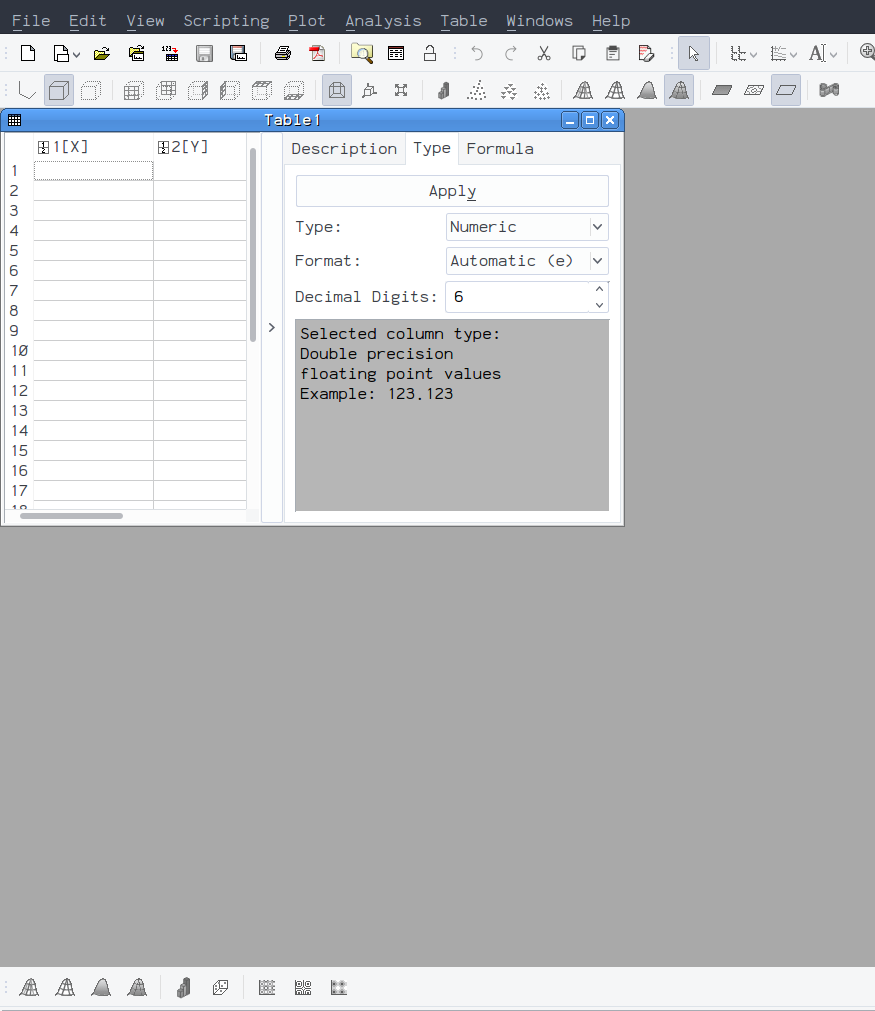
\includegraphics[width=0.6\textwidth]{basico/1mostra.png}

    \caption{Tela inicial do \software}
    \label{fig:basico:mostragem}
\end{figure}


% \subsection{Alterando a Fonte Padrão}

%     Como a fonte padrão do \texttt{Origin} não funciona muito bem com acentos e outros símbolos da língua portuguesa, é recomendado utilizar outra fonte nos gráficos. Nos exemplos a seguir será aplicada a fonte \texttt{Times New Roman}, que funciona com os acentos gráficos e é facilmente encontrada em qualquer máquina com \texttt{Windows}. Todo o processo é bem simples e está especificado na figura \ref{fig:basico:mudar_fontes}.

%     \begin{figure}[htbp]
%         \centering
%         \begin{subfigure}{0.45\textwidth}
%             \centering
%             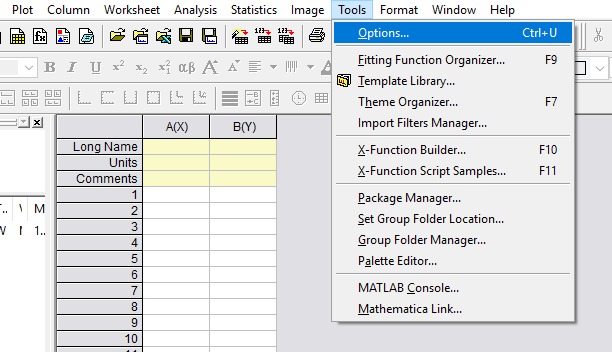
\includegraphics[width=\textwidth]{basico/2options.png}

%             \caption{Acesso às opções}
%             \label{fig:basico:options}
%         \end{subfigure}
%         ~
%         \begin{subfigure}{0.45\textwidth}
%             \centering
%             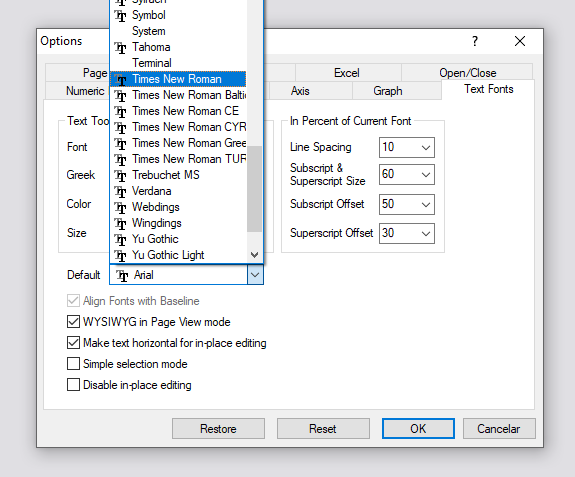
\includegraphics[width=\textwidth]{basico/3fonts.png}

%             \caption{Opção de fontes}
%             \label{fig:basico:fontes}
%         \end{subfigure}
%         \caption{Mudando a fonte padrão}
%         \label{fig:basico:mudar_fontes}
%     \end{figure}


\subsection{Importando os Dados} \label{sec:basico:import}

    Assim como no \texttt{Origin}, o \software tem um gerenciador de tabelas prórpio, apesar de simplificado, onde os dados podem ser apenas copiados e colados de outra tabela do \texttt{Excel}, \texttt{Google Planilhas}, \texttt{LibreOffice Calc} ou outra ferramenta do tipo. Quando os dados são importados assim, a formatação das linhas e colunas se matém. Outra opção é importar de arquivos de texto de campos separados, como o \texttt{CSV} e suas variações.

    \begin{lembrete}
        Cuidado com o separador decimal. Em português e outras línguas europeias é mais comum encontrar a vírgula [\texttt{,}] como separador da parte decimal do número, enquanto nos países anglofônicos é o ponto final [\texttt{.}] que define a parte fracionária e a vírgula serve para separar os milhares. Dependendo da configuração do \software e da formatação original dos dados, isso pode causar problemas de importação e os dados serão tratados como tipo \texttt{Text}.
    \end{lembrete}


\subsection{Configurando as Colunas} \label{sec:basico:renome}

    Por padrão, as colunas são criadas com letras com números. Para mudar isso, basta alterar as propriedades da coluna, que fica na parte direita da janela da tabela, como na figura \ref{fig:basico:colnome}. Além disso, se você importar os dados de um arquivo \texttt{.csv}, é possível utilizar a primeira linha como nome da coluna, o \textit{header}.

    Outra coisa importante é o tipo de dado da coluna. Para a construção dos gráficos, o desejado normalmente são dados de tipos numéricos ou, às vezes, datas. Porém, é possível que os dados estejam sendo tratados como texto, como no problema descrito na seção \nameref{sec:basico:import}. Por isso, deve se ter o cuidado de escolher o tipo certo, seguindo a figura \ref{fig:basico:coltipo}, antes e depois de importar os valores.

    \begin{figure}[htbp]
        \begin{subfigure}{0.45\textwidth}
            \centering
            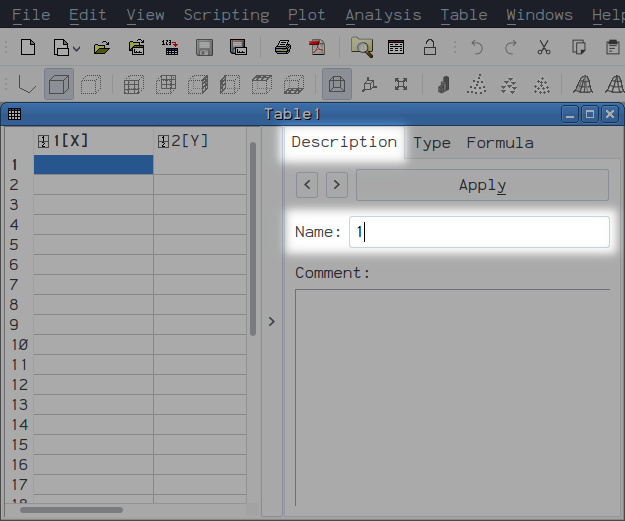
\includegraphics[width=\textwidth]{basico/3colnome.png}

            \caption{Nome da coluna}
            \label{fig:basico:colnome}
        \end{subfigure}
        ~
        \centering
        \begin{subfigure}{0.45\textwidth}
            \centering
            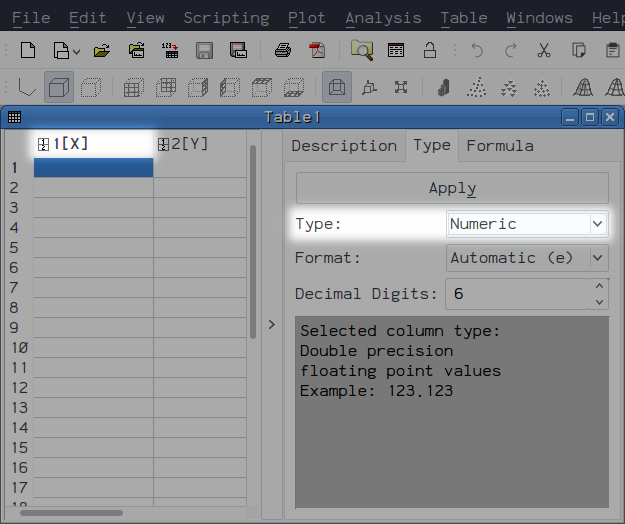
\includegraphics[width=\textwidth]{basico/2coltype.png}

            \caption{Tipo dos dados da coluna}
            \label{fig:basico:coltipo}
        \end{subfigure}
        \caption{Configuração da coluna selecionada}
        \label{fig:basico:config}
    \end{figure}

    \begin{lembrete}
        Lembre-se de pressionar o botão \texttt{Apply} sempre que alterar alguma propriedade da coluna, para realizar as alterações.
    \end{lembrete}


    \section{Apresentação dos Dados} \label{sec:reta}
        % \begin{figure}[htbp]
    \centering
    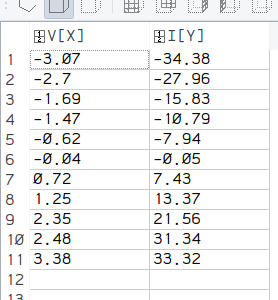
\includegraphics[width=0.35\textwidth]{reta/1dados.png}

    \caption{Dados de corrente por tensão, gerados por computador}
    \label{fig:reta:dados}
\end{figure}

Nesta seção, será tomado como exemplo a relação de corrente e tensão em um resistor, dado de forma teórica pela relação (\ref{eq:resist}). Por mais que os dados usados aqui sejam os da figura \ref{fig:reta:dados}, essa parte de apresentação de dados é importante para todos os tipos de análise, em especial, para dados coletados manualmente, como é o caso da maioria dos experimentos da disciplina de \texttt{F 329}.

\begin{equacao} \label{eq:resist}
    I = \frac{1}{R} ~ V
\end{equacao}


\subsection{Dados Pontuais}

    Normalmente, quando se trata de dados pontuais, às vezes é importante mostrar esses dados, além de em alguma tabela, no gráfico também. O modo de se fazer isso no \software é com a funcionalidade \texttt{Scatter} (figura \ref{fig:reta:scatter}).

    \begin{figure}[htbp]
        \centering
        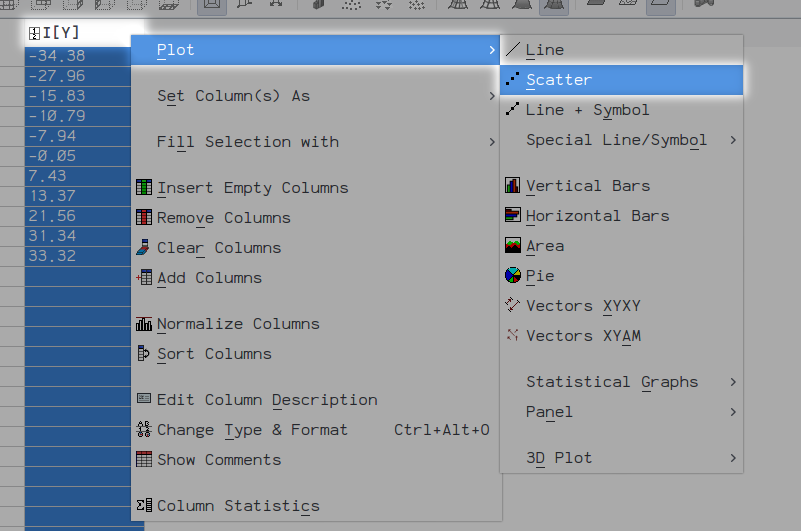
\includegraphics[width=0.6\textwidth]{reta/2scatter.png}

        \caption{\texttt{Scatter}}
        \label{fig:reta:scatter}
    \end{figure}

    \begin{figure}[htbp]
        \centering
        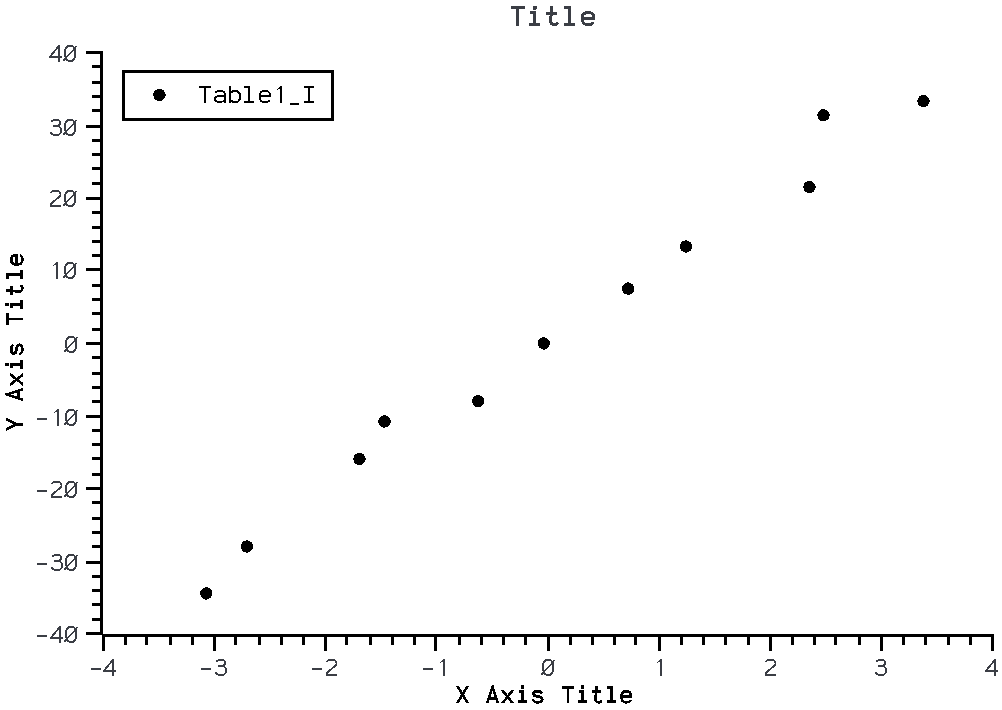
\includegraphics[width=0.5\textwidth]{reta/1linscatter.pdf}

        \caption{Resultado do \texttt{Scatter}}
        \label{fig:reta:linscatter}
    \end{figure}


\subsection{Tratamento da Legenda}

    O \software gera uma legenda padrão para os elementos desenhados no gráfico. O ideal é alterá-las para serem mais informativas. As legendas também podem ser reposicionadas apenas arrastando-as. Por padrão, o plano de fundo da legenda é transparente, mas é recomendável mudar para um plano de fundo preenchido em branco ou qualquer que seja a cor de fundo do gráfico.

    \begin{figure}[htbp]
        \centering
        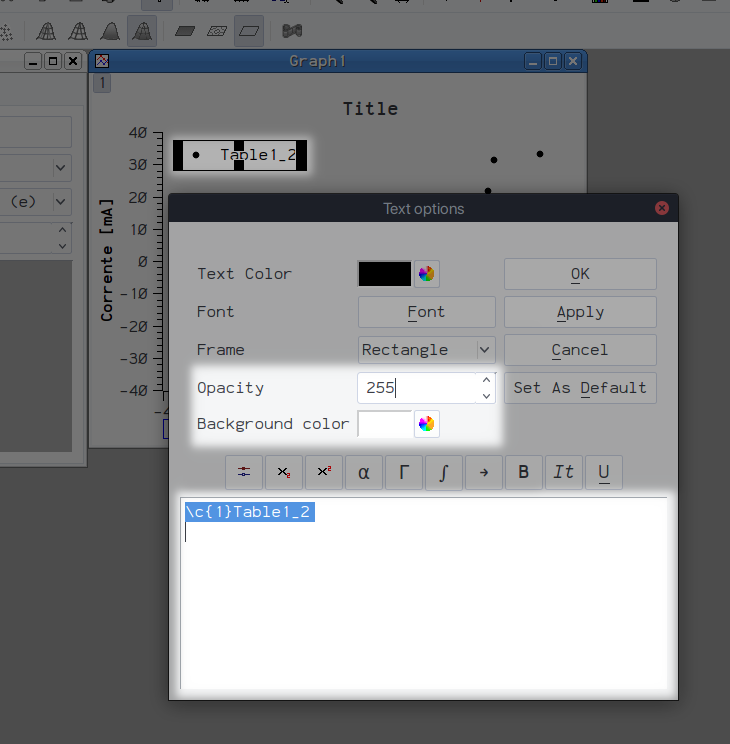
\includegraphics[width=0.5\textwidth]{reta/3legenda.png}

        \caption{Alterando o texto da legenda}
        \label{fig:reta:legenda}
    \end{figure}


\subsection{Formatação dos Eixo e do Título}

    Diferente do \texttt{Origin}, o \software não coloca nada nos texto do gráfico, então isso deve ser feito manualmente, como é visto nas figuras \ref{fig:reta:eixo} e \ref{fig:reta:titulo}.

    \begin{figure}[htbp]
        \centering
        \begin{subfigure}{0.45\textwidth}
            \centering
            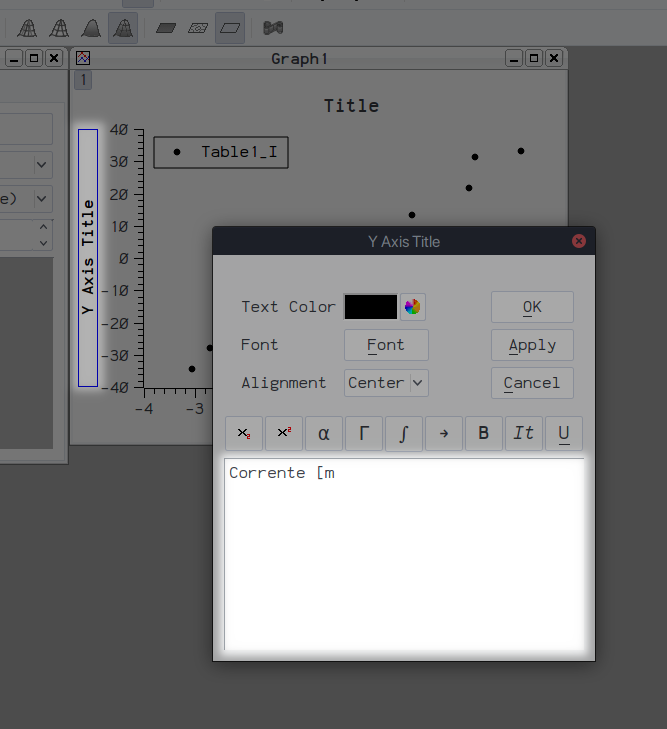
\includegraphics[width=\textwidth]{reta/4eixos.png}

            \caption{Alterando dos nomes dos eixos}
            \label{fig:reta:eixo}
        \end{subfigure}
        ~
        \begin{subfigure}{0.45\textwidth}
            \centering
            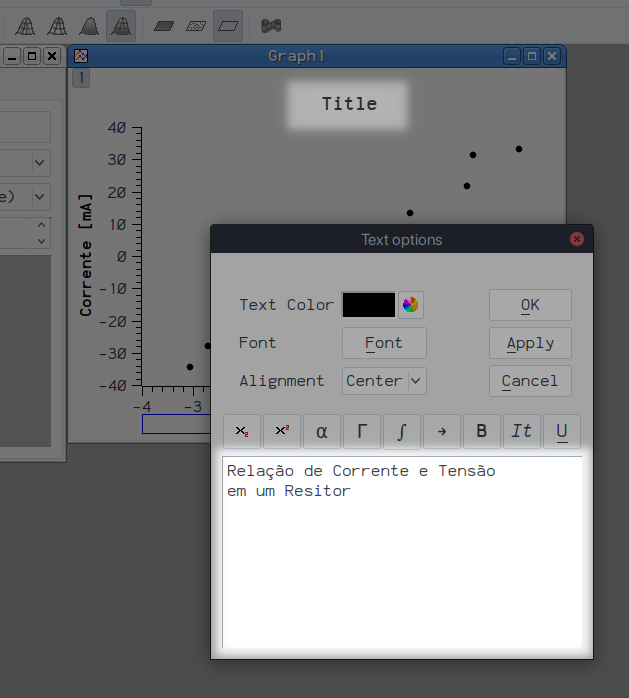
\includegraphics[width=\textwidth]{reta/4titulo.png}

            \caption{Mudança do título}
            \label{fig:reta:titulo}
        \end{subfigure}
        \caption{Opções dos textos principais do gráfico}
        \label{fig:reta:textos}
    \end{figure}


\subsection{Linhas de Grid}

    Para ler melhor os eixos do gráfico, é possível colocar linhas de \textit{grid} acompanhando os valores principais.

    \begin{figure}[htbp]
        \centering
        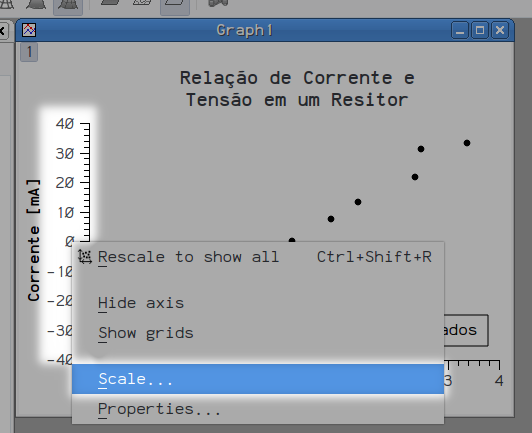
\includegraphics[width=0.55\textwidth]{reta/5gridopt.png}

        \caption{Acesso as opções de formatação de linha de acompanhamento dos eixos}
        \label{fig:reta:gridopt}
    \end{figure}

    No material, serão utilizadas linhas principais horizontais e verticais, que serão em tracejados em cinza escuro, sem linhas secundárias. Essas configurações podem e devem ser alteradas para cada gráfico, dependendo da facilidade e da importância da leitura dos valores.

    \begin{figure}[htbp]
        \centering
        \begin{subfigure}{0.45\textwidth}
            \centering
            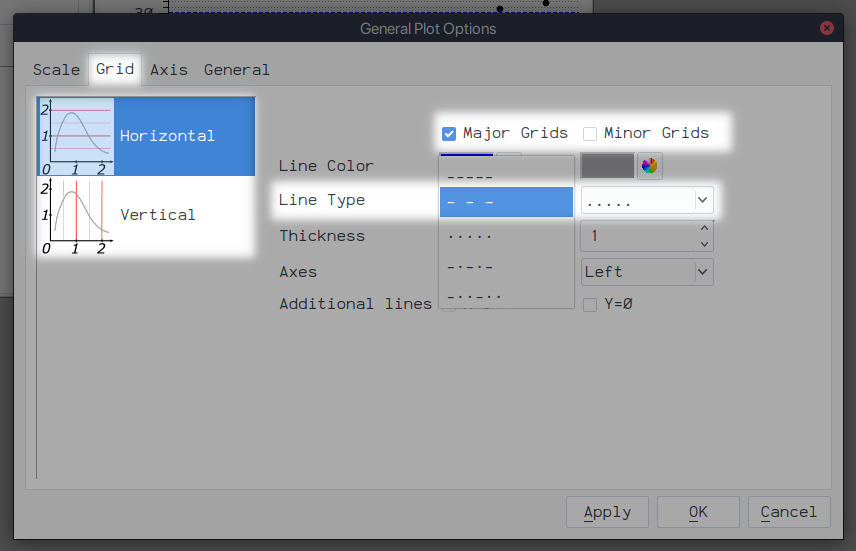
\includegraphics[width=\textwidth]{reta/6grid.png}

            \caption{Opções dos eixos (aba \texttt{Grid})}
            \label{fig:reta:grid}
        \end{subfigure}
        ~
        \begin{subfigure}{0.45\textwidth}
            \centering
            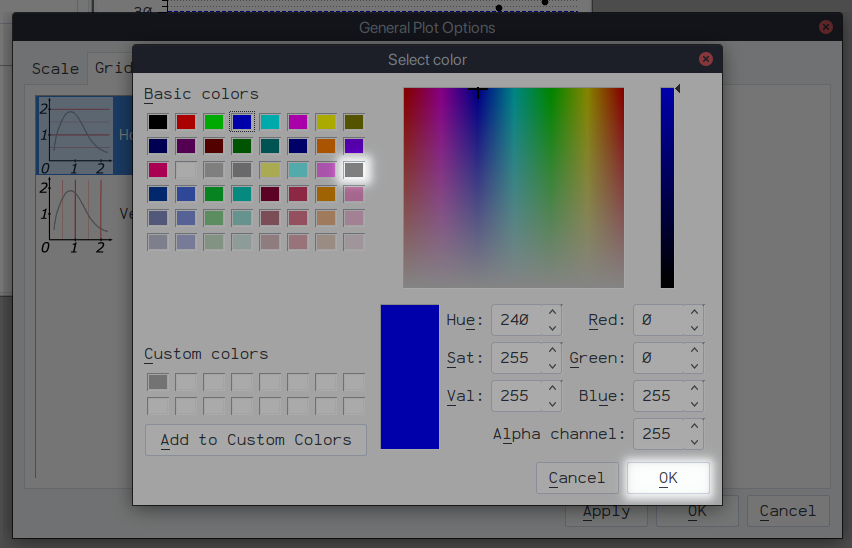
\includegraphics[width=\textwidth]{reta/6cor.png}

            \caption{Mudança de cor das linhas}
            \label{fig:reta:gridcor}
        \end{subfigure}
        \caption{Opções de linhas de \textit{grid}}
        \label{fig:reta:opcoes_eixo}
    \end{figure}


\subsection{Resultado}

    \begin{figure}[htbp]
        \centering
        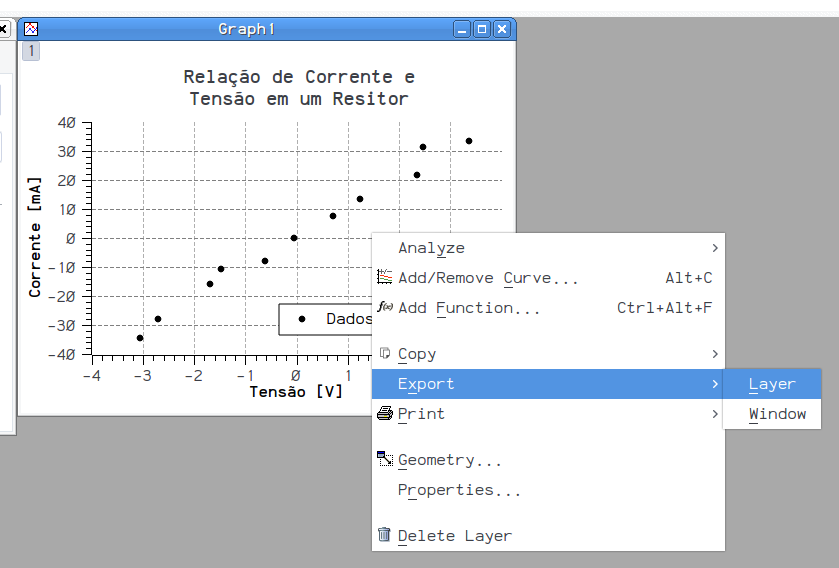
\includegraphics[width=0.5\textwidth]{reta/7save.png}

        \caption{Salvando o gráfico resultante}
        \label{fig:reta:salvar}
    \end{figure}

    \begin{figure}[H]
        \centering
        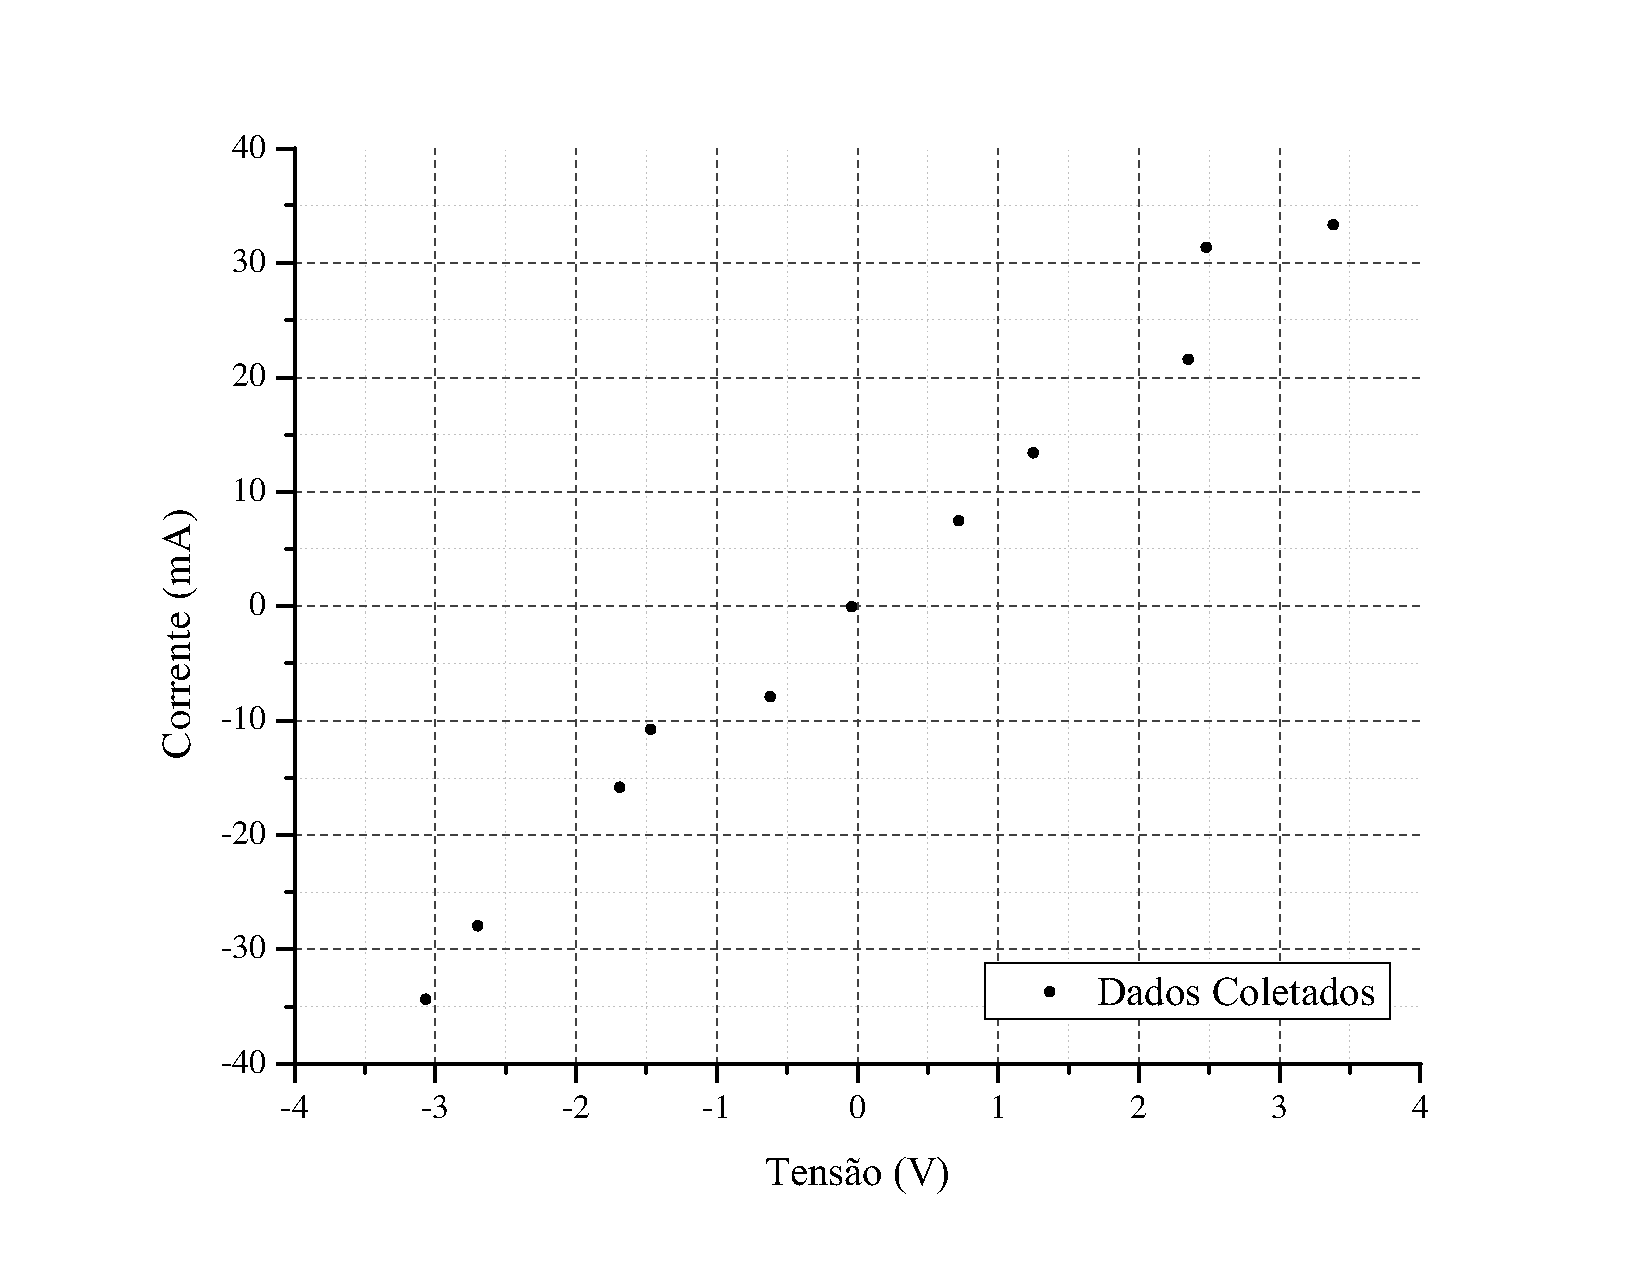
\includegraphics[width=0.6\textwidth]{reta/2gridlinscat.pdf}

        \caption{Gráfico de exemplo de formatação}
        \label{fig:reta:gridlinscat}
    \end{figure}



    \section{Regressão Linear} \label{sec:regres}
        % É muito comum aparecer algum tipo de relação linear entre os dados. Nesse tipo de relação costuma-se aplicar técnicas de regressão, normalmente mínimos quadrados, para encontrar a melhor reta que representa esses dados.

Pelo alinhamento dos pontos da seção \nameref{sec:reta} e pela equação teórica \ref{eq:resist}, fica clara a possibilidade de se aplicar uma regressão linear e, portanto, os dados continuarão os mesmos nessa seção.

\subsection{Configuração da Regressão}

    A regressão normalmente é feita pelas opções \textbf{Analysis: Fitting: Fit Linear}. Isso abre a janela de opções (figura \ref{fig:regres:opt}). Quando terminada a regressão, aparecerá uma janela perguntando para mudar de aba, mas por enquanto é melhor continuar nesta aba.

    Existem outras formas de regressão além da linear, mas elas não serão abordadas nesta matéria.

    \begin{figure}[htbp]
        \centering
        \begin{subfigure}{0.60\textwidth}
            \centering
            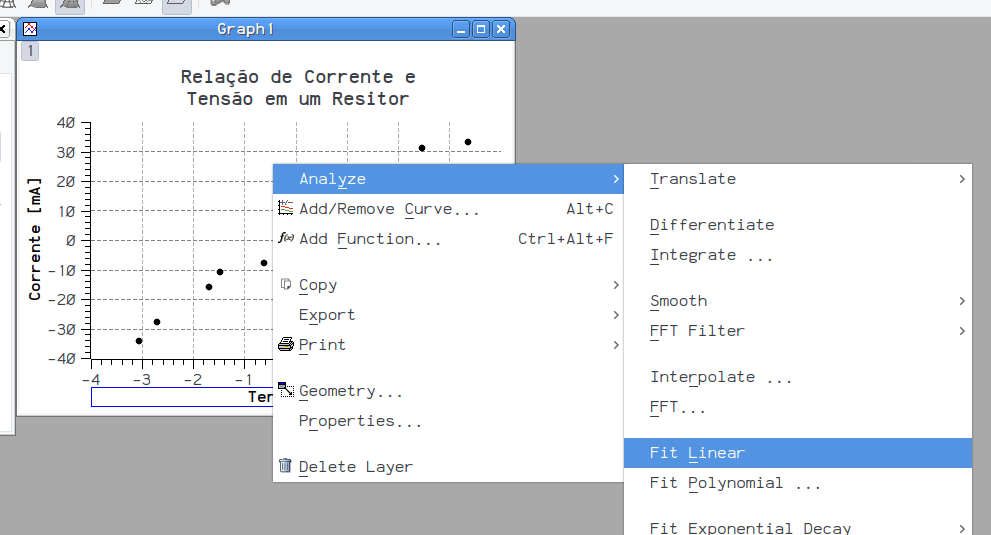
\includegraphics[width=\textwidth]{regres/1regpath.png}

            \caption{Acessando as opções de regressão}
            \label{fig:regres:path}
        \end{subfigure}
        ~
        \begin{subfigure}{0.35\textwidth}
            \centering
            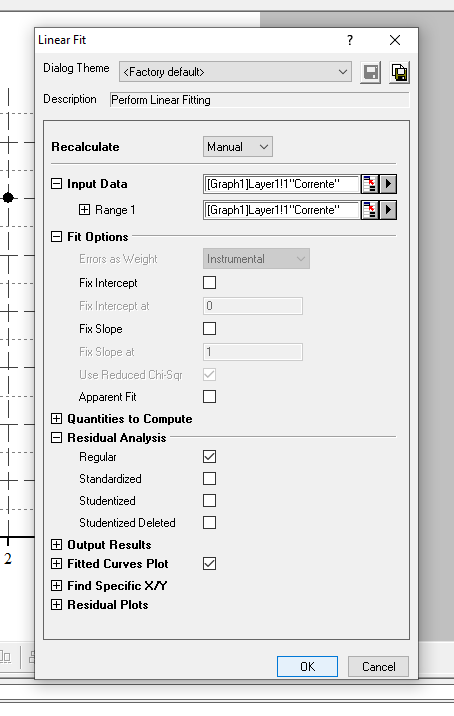
\includegraphics[width=\textwidth]{regres/2regopt.png}

            \caption{Opções de regressão}
            \label{fig:regres:opt}
        \end{subfigure}
        \caption{Configuração da regressão}
        \label{fig:regres:config}
    \end{figure}


    \subsection{Tabela dos Coeficientes}

    Por padrão, os coeficientes da regressão aparecem na tabela como está na figura \ref{fig:regres:coefspadrao}. Ao acessar a tabela \texttt{Table1} na parte esquerda do programa, é possível modificar essa tabela. Após a modificação, é importante apertar \texttt{Update Table} para atualizar a visualização no gráfico.

    \begin{figure}[htbp]
        \centering
        \begin{subfigure}{0.45\textwidth}
            \centering
            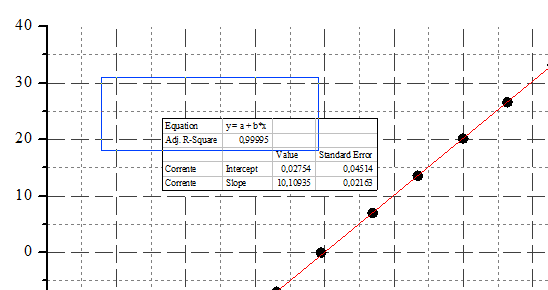
\includegraphics[width=\textwidth]{regres/4mover.png}

            \caption{Tabela padrão de coeficientes da regressão}
            \label{fig:regres:coefspadrao}
        \end{subfigure}
        ~
        \begin{subfigure}{0.50\textwidth}
            \centering
            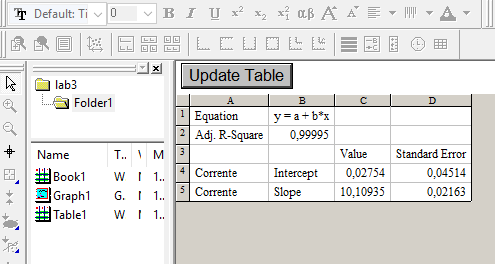
\includegraphics[width=\textwidth]{regres/5tabcoefs.png}

            \caption{Configuração da tabela de coeficientes}
            \label{fig:regres:tabcoefs}
        \end{subfigure}
        \caption{Tabela de coeficientes da regressão}
        \label{fig:regres:coefs}
    \end{figure}


\subsection{Formatação dos Coeficientes}

    Por padrão, os coeficientes da regressão aparecem na tabela como está na figura \ref{fig:regres:coefspadrao}. Ao acessar a aba \texttt{Table1} na parte esquerda do programa, é possível modificar essa tabela.

    Na figura \ref{fig:regres:renome2}, aparece o padrão que será seguido neste tutorial para essa tabela de coeficientes. As dimensões da tabela (figura \ref{fig:regres:tamanhos}), que mudam para cada caso, não seguirão nenhum padrão aqui.

    \begin{figure}[htbp]
        \centering
        \begin{subfigure}{0.45\textwidth}
            \centering
            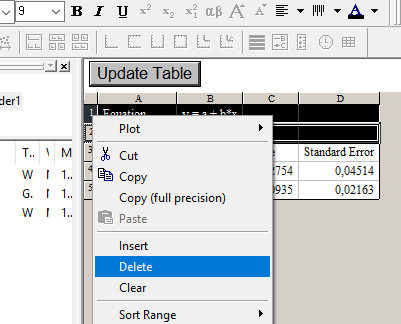
\includegraphics[width=\textwidth]{regres/6del1.png}

            \caption{Removendo as linhas superiores}
            \label{fig:regres:del1}
        \end{subfigure}
        ~
        \begin{subfigure}{0.450\textwidth}
            \centering
            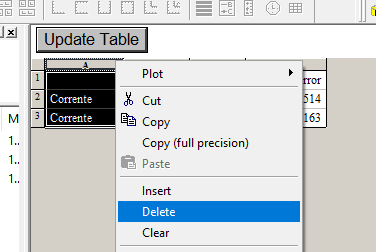
\includegraphics[width=\textwidth]{regres/7del2.png}

            \caption{Removendo as colunas de descrição}
            \label{fig:regres:del2}
        \end{subfigure}
        \caption{Reduzindo a tabela de coeficientes}
        \label{fig:regres:del}
    \end{figure}

    \begin{figure}[htbp]
        \centering
        \begin{subfigure}{0.45\textwidth}
            \centering
            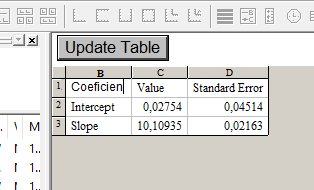
\includegraphics[width=\textwidth]{regres/8renome.png}

            \caption{Renomeando os campos}
            \label{fig:regres:renome1}
        \end{subfigure}
        ~
        \begin{subfigure}{0.450\textwidth}
            \centering
            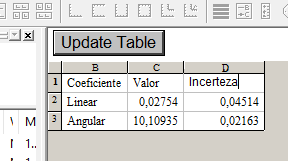
\includegraphics[width=\textwidth]{regres/9renomeado.png}

            \caption{Campos da tabela depois de renomeados}
            \label{fig:regres:renome2}
        \end{subfigure}
        \caption{Renomeando os campos da tabela de coeficientes da regressão}
        \label{fig:regres:renome}
    \end{figure}

    \begin{figure}[htbp]
        \centering
        \begin{subfigure}{0.5\textwidth}
            \centering
            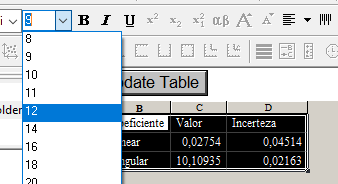
\includegraphics[width=\textwidth]{regres/10fontetam.png}

            \caption{Ajustando o tamanho da fonte}
            \label{fig:regres:fontetam}
        \end{subfigure}
        ~
        \begin{subfigure}{0.40\textwidth}
            \centering
            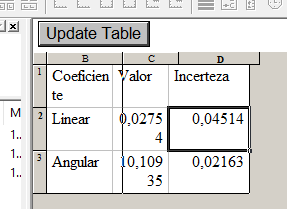
\includegraphics[width=\textwidth]{regres/11colunatam.png}

            \caption{Ajustando a largura da coluna}
            \label{fig:regres:colunatam}
        \end{subfigure}
        \caption{Ajustando as dimensões da tabela de coeficientes da regressão}
        \label{fig:regres:tamanhos}
    \end{figure}

    \begin{figure}[htbp]
        \centering
        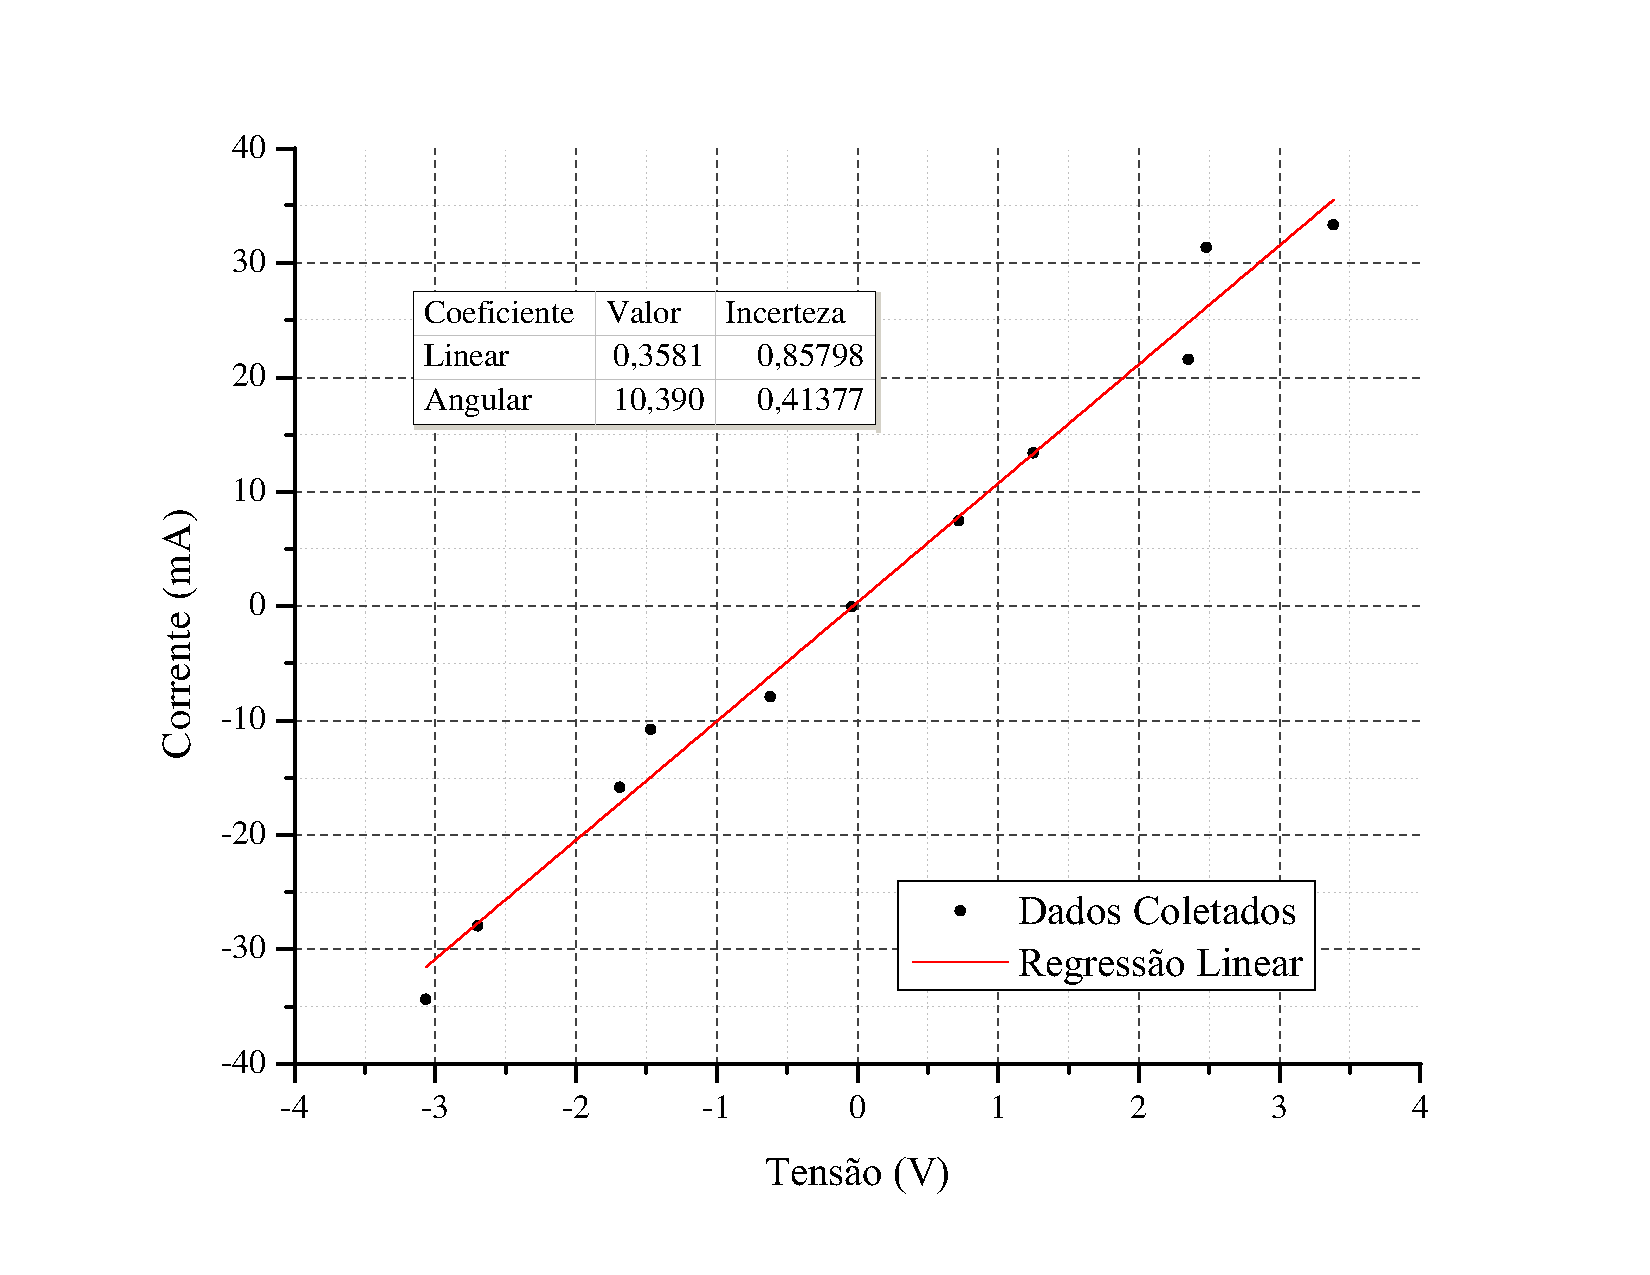
\includegraphics[width=0.8\textwidth]{regres/z1parcial.pdf}

        \caption{Exemplo de regressão linear para a relação de corrrente por tensão}
        \label{fig:regres:semifinal}
    \end{figure}


\subsection{Pontos Fora da Reta}

    Podemos ver que a regressão (figura \ref{fig:regres:semifinal}) resultou em alguns pontos que não ficaram muito próximos a reta encontradada. Esses pontos podem ser marcados para serem ignorados na regressão, como mostra a figura \ref{fig:regres:outliers}. Note que os pontos marcados passam a ser coloridos em vermelho (figura \ref{fig:regres:recalc}).

    \begin{figure}[htbp]
        \centering
        \begin{subfigure}{0.35\textwidth}
            \centering
            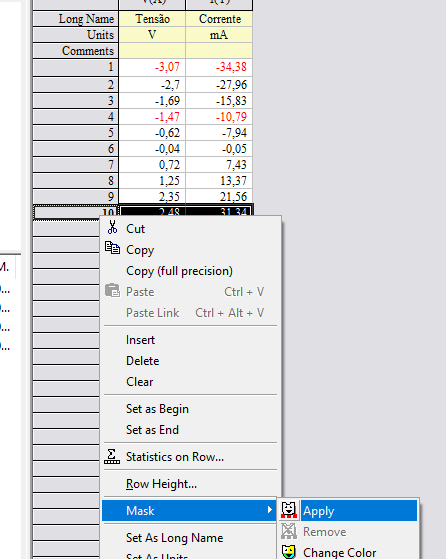
\includegraphics[width=\textwidth]{regres/12remov.png}

            \caption{Marcando os pontos a serem ignorados}
            \label{fig:regres:mask}
        \end{subfigure}
        ~
        \begin{subfigure}{0.35\textwidth}
            \centering
            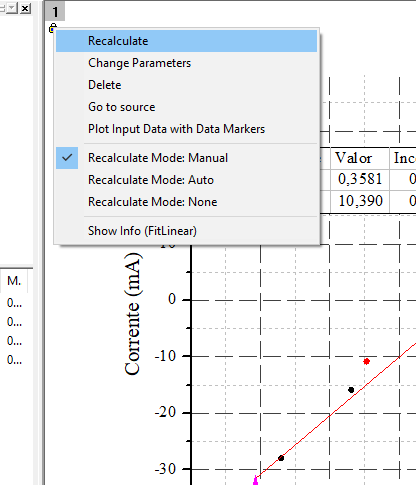
\includegraphics[width=\textwidth]{regres/13recalc.png}

            \caption{Recalculando os coeficientes da regressão}
            \label{fig:regres:recalc}
        \end{subfigure}
        \caption{Removendo pontos selecionados da regressão}
        \label{fig:regres:outliers}
    \end{figure}


\subsection{Resultado}

    \begin{figure}[htbp]
        \centering
        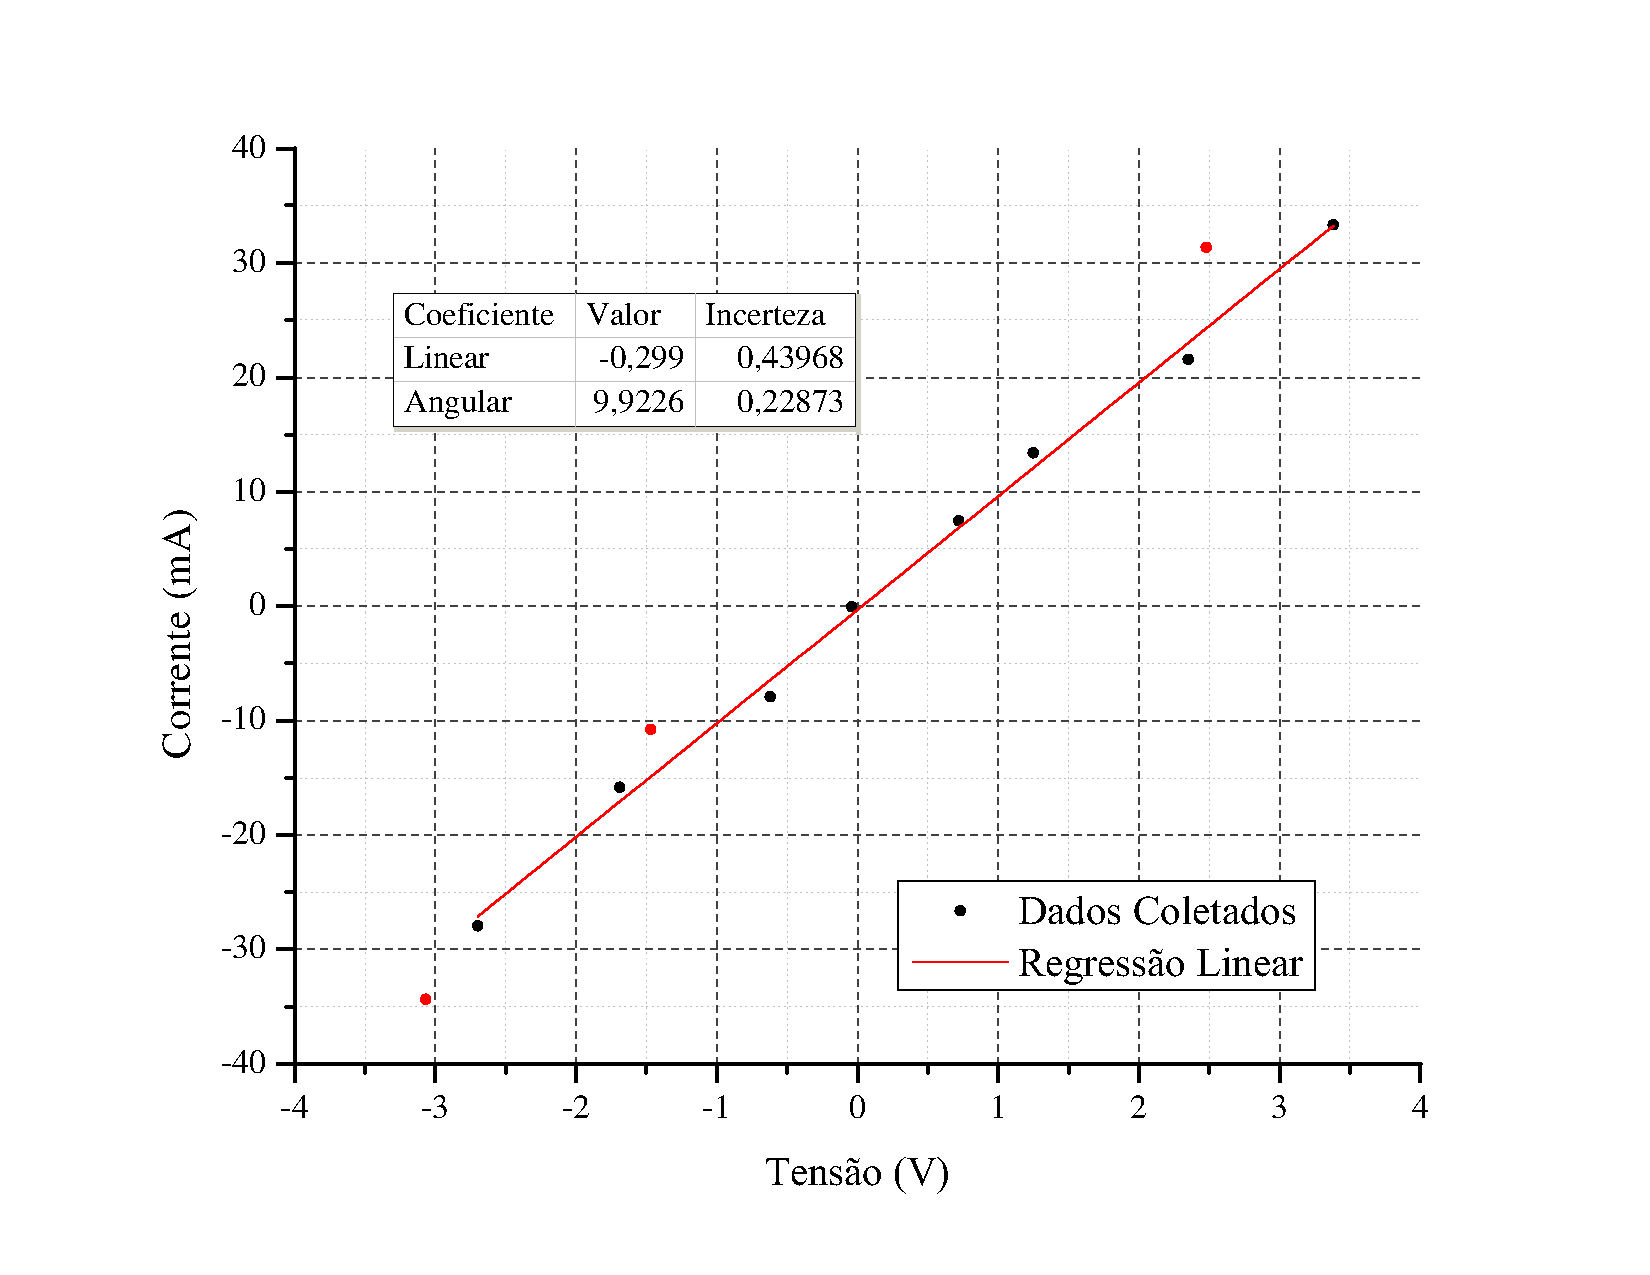
\includegraphics[width=0.8\textwidth]{regres/z2final.pdf}

        \caption{Exemplo de regressão linear com pontos ignorados}
        \label{fig:regres:final}
    \end{figure}

    Observando o resultado na figura \ref{fig:regres:final}, a nova regressão com os pontos ignorados obteve uma redução significativa na incerteza dos coeficientes. Isso indica que a remoção de \textit{outliers} é um passo importante na medição, mas deve ser feito com cuidado. A retirada de pontos válidos para a regressão pode reduzir não só a exatidão da medida, mas até mesmo a precisão, pela maneira como o cálculo da regressão é feito.


    \section{Barras de Incerteza} \label{sec:incert}
        % Como exemplo para a aplicação de barras de incerteza, continuaremos com os mesmo dados da seção \nameref{sec:reta}, porém agora com as incertezas associadas a cada medida, que foram criadas, novamente, com o auxílio de um computador, e podem ser vistas na figura \ref{fig:incert:dados}.


\subsection{Adicionando Colunas}

    \begin{figure}[htbp]
        \centering
        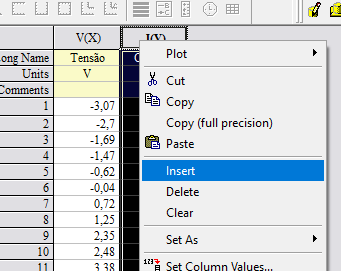
\includegraphics[width=0.4\textwidth]{incert/1insert.png}

        \caption{Inserindo novas colunas}
        \label{fig:incert:colunas}
    \end{figure}

    Para adicionar a incertezas, é preciso gerar novas colunas nas tabelas, como mostra a figura \ref{fig:incert:colunas}, lembrando sempre de formatá-las como na seção \nameref{sec:basico:renome}. A tabela com os dados de incerteza deve ficar algo parecido com a figura \ref{fig:incert:dados}.

    \begin{figure}[htbp]
        \centering
        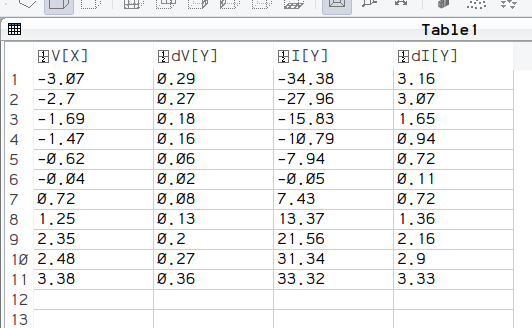
\includegraphics[width=0.5\textwidth]{incert/2dados.png}

        \caption{Dados atualizados com as incertezas}
        \label{fig:incert:dados}
    \end{figure}


\subsection{Tipo das Novas Colunas}

    \begin{figure}[htbp]
        \centering
        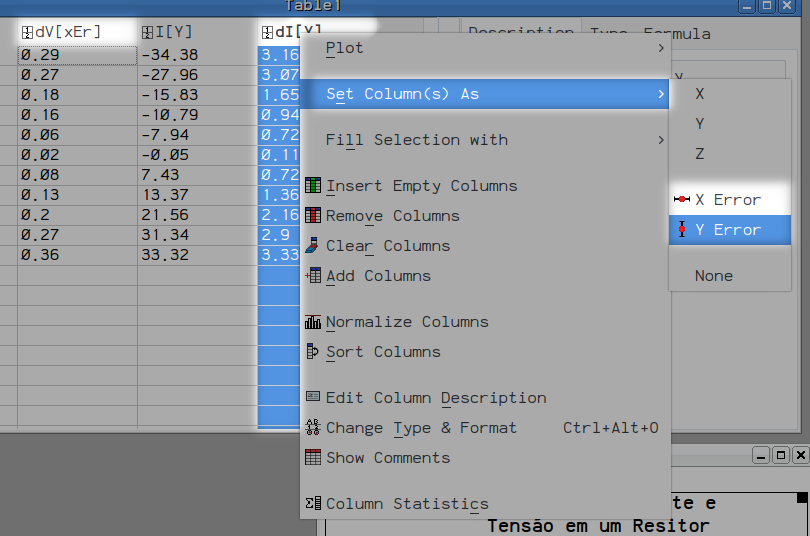
\includegraphics[width=0.6\textwidth]{incert/3xyer.png}
        \caption{Mudando o tipo das novas colunas para relacionar com os valores das medidas}
        \label{fig:incert:tipos}
    \end{figure}


\subsection{Resultados}

    A funcionalidade \texttt{Scatter}, quando selecionada com as colunas de incerteza, gera o gráfico da figura \ref{fig:incert:preresultado}.

    \begin{figure}[htbp]
        \centering
        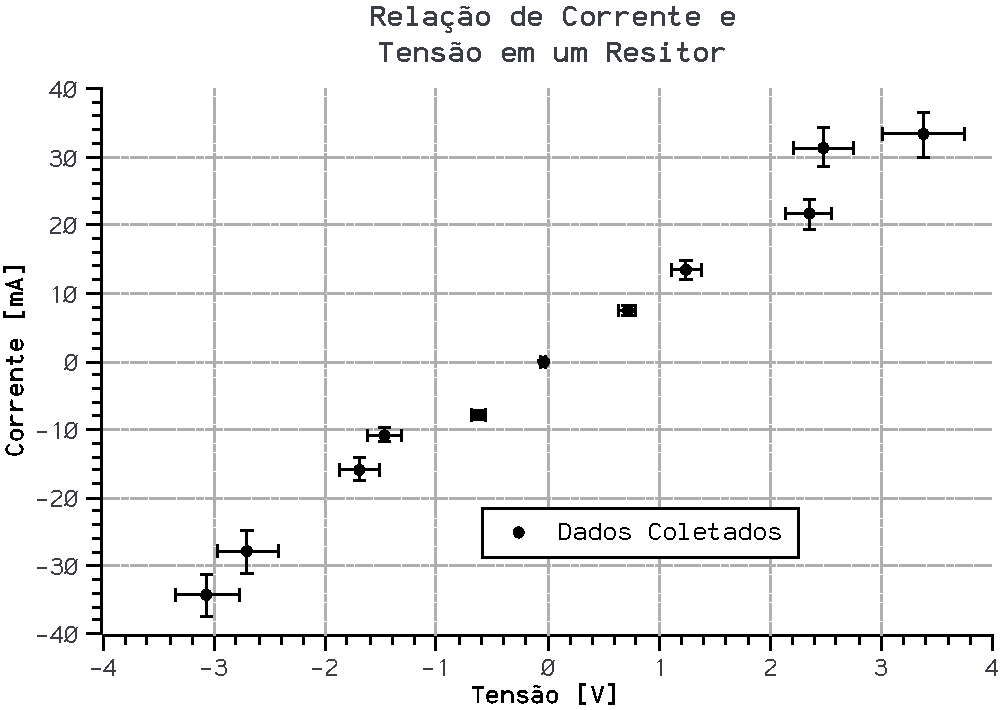
\includegraphics[width=0.6\textwidth]{incert/preresultado.pdf}

        \caption{Gráfico de corrente por tensão com as incertezas de cada medida}
        \label{fig:incert:preresultado}
    \end{figure}

    Entretanto, se for aplicada a formatação da seção \nameref{sec:reta} e a regressão linear, como na seção \nameref{sec:regres}, o resultado deveria ficar semelhante a figura \ref{fig:incert:resultado}, cujos coeficientes são $B = 0.34 \pm 0.11$ e $A = 9.8 \pm 0.3$.

    \begin{figure}[htbp]
        \centering
        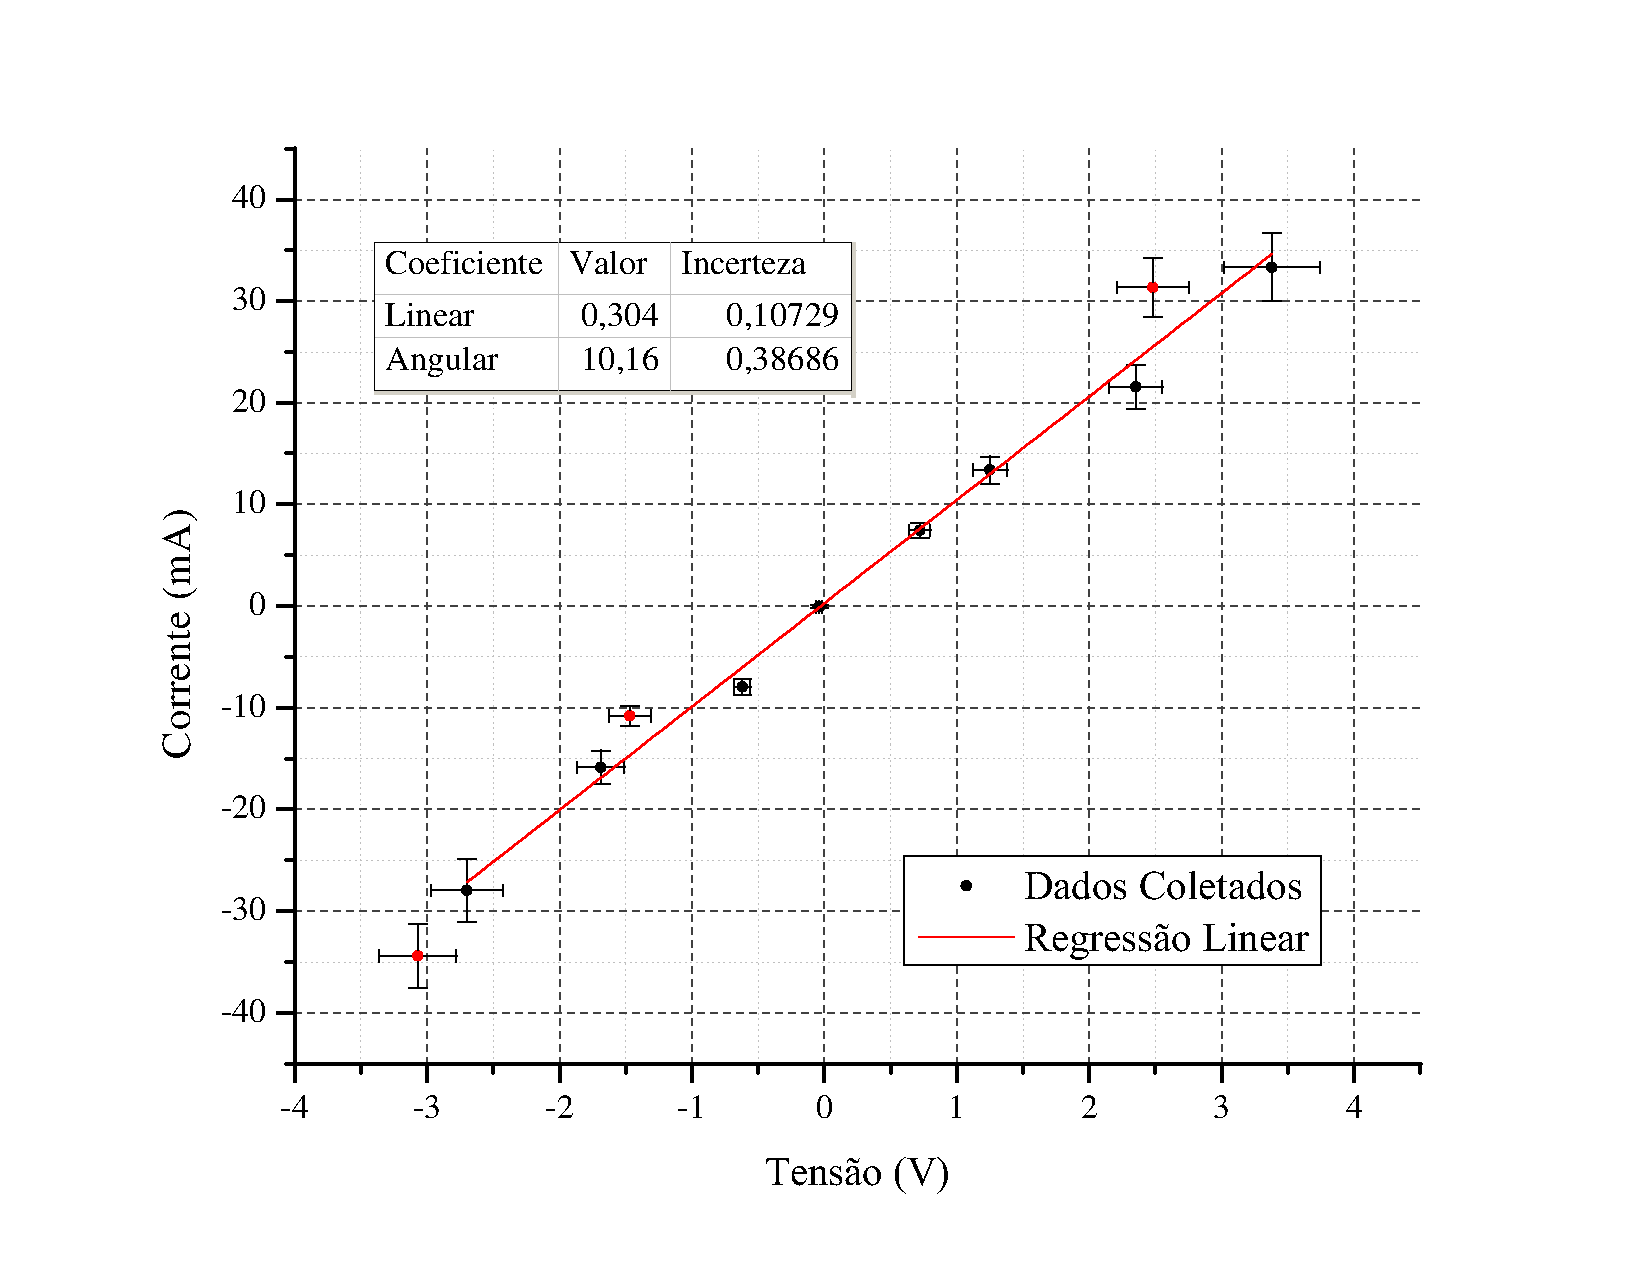
\includegraphics[width=0.6\textwidth]{incert/resultado.pdf}

        \caption{Gráfico formatado, com barras de incerteza e regressão linear}
        \label{fig:incert:resultado}
    \end{figure}

    \begin{nota}
        Note que os coeficientes $A$ e $B$ da regressão em \ref{fig:incert:resultado}, tanto em seus valores quanto nas suas incertezas, são levemente diferentes dos da figura \ref{fig:regres:coefs}, mesmo com os dados numéricos idênticos. A diferença aqui se deve as incertezas dos dados, que agora estão sendo levadas em conta no cálculo da regressão.
    \end{nota}


    \section{Escala Logarítmica} \label{sec:escala}
        Várias vezes, no entanto, os dados não apresentam relação linear. Nesses casos, é importante encontrar alguma técnica de linearização que transforma os dados para novos valores dependentes, mas que se relacionam de maneira linear. Algo como a relação \ref{eq:linearizacao}.

\begin{equacao} \label{eq:linearizacao}
    f(x, y) = a + b ~ g(x, y)
\end{equacao}

Dentre as técnicas mais comuns, muitas envolvem a aplicação de logaritmos para linearizar alguma relação de potência de $x$, isto é, nos casos de $y \propto x^k$, ou alguma relação exponencial, $y \propto k^x$. Para esses casos, é comum a utilização de escala logarítmica na intenção de se observar melhor os dados, em que $f(x, y) = \log(y)$ e $g(x, y) = \log(x)$.


\subsection{Gráfico Log-Log}

    \begin{figure}[htbp]
        \centering
        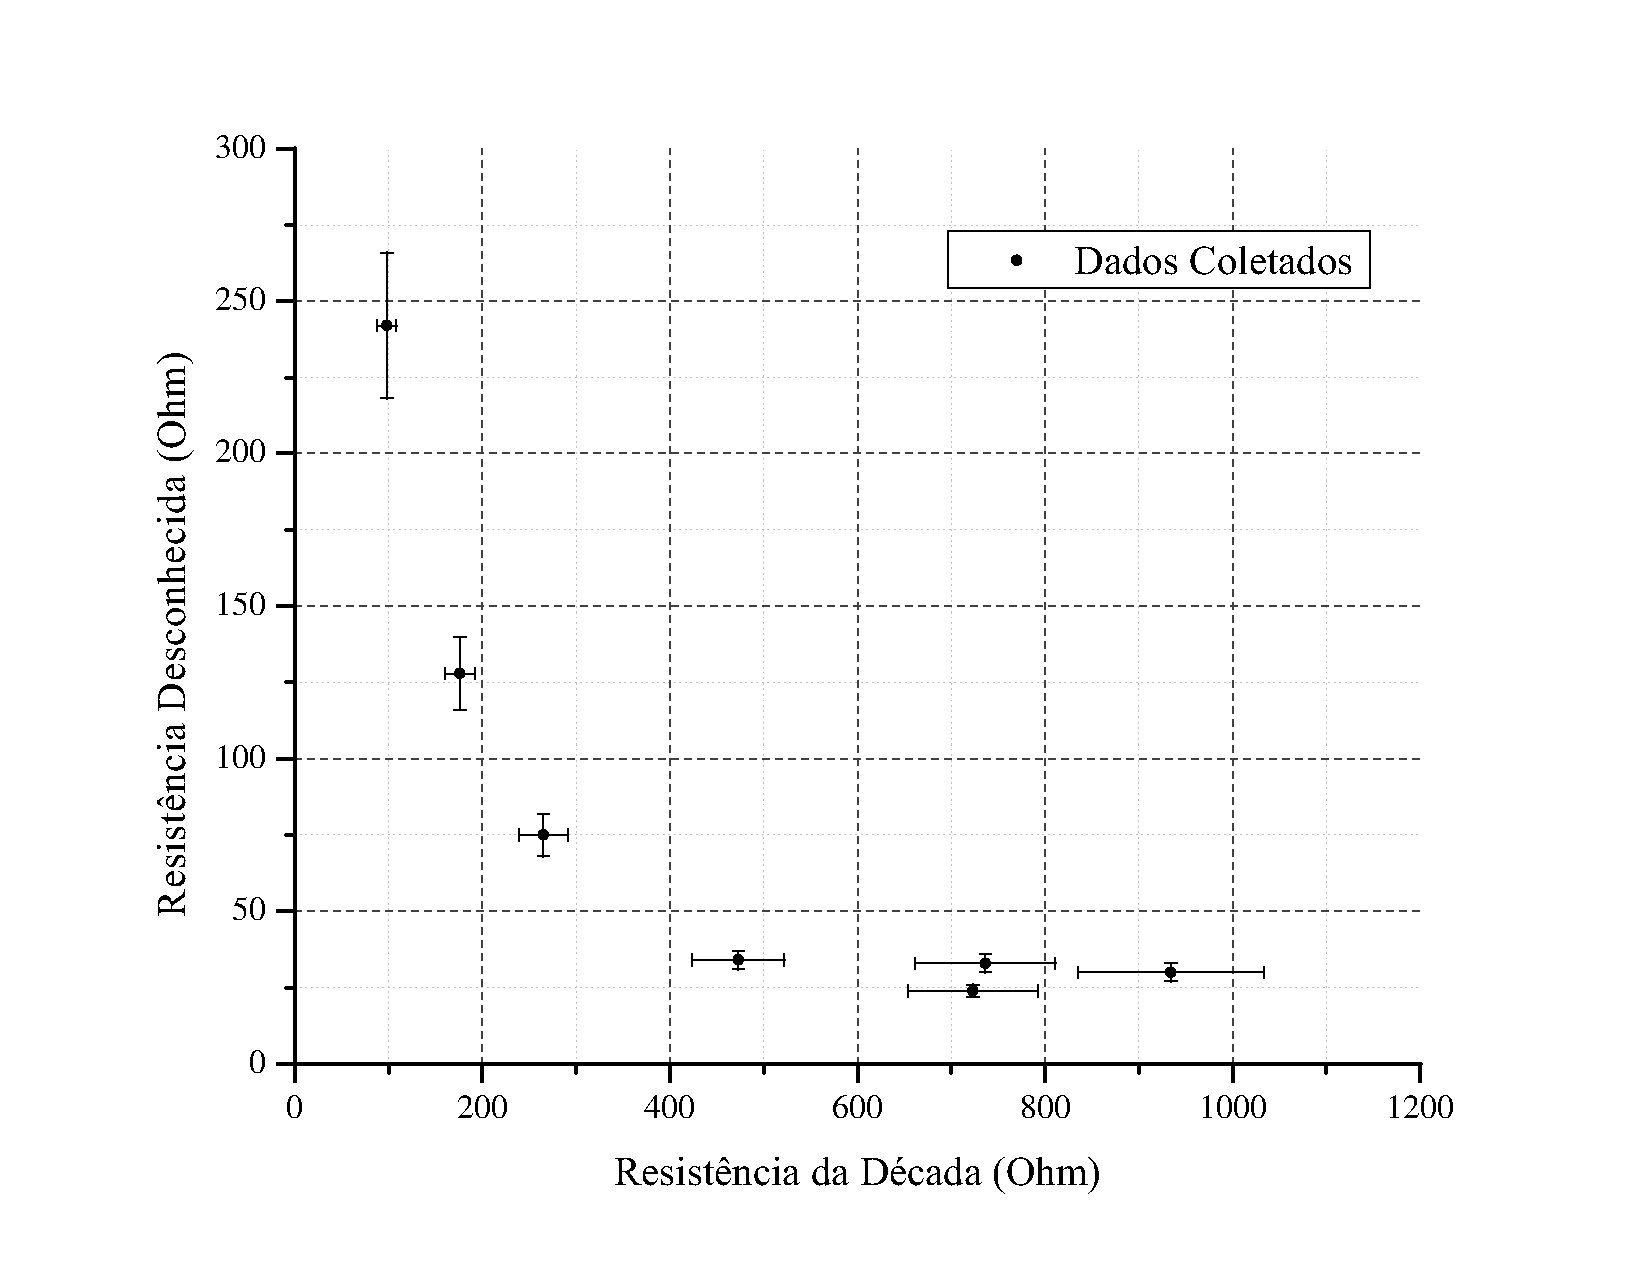
\includegraphics[width=0.6\textwidth]{escala/1dados.pdf}

        \caption{Gráfico da relação da ponte de Wheatstone (\ref{eq:wheatstone})}
        \label{fig:escala:loglog:dados}
    \end{figure}

    \begin{equacao} \label{eq:wheatstone}
        R_x = \frac{R_1 R_2}{R_d}
    \end{equacao}

    Se imaginarmos os dados do gráfico \ref{fig:escala:loglog:dados} como parte de um caso da ponte de Wheatstone dado pela equação \ref{eq:wheatstone}, sendo $R_d$ a resistência da década e $R_x$ a resistência desconhecida, podemos aplicar a seguinte técnica de linearização:

    \begin{align*}
        \log(R_x)
            &= \log\left(R_1 R_2 ~ (R_d)^{-1}\right) \\
            &= \log(R_1 R_2) + \log\left((R_d)^{-1}\right) \\
            &= \log(R_1 R_2) - \log(R_d)
    \end{align*}

    Portanto, podemos montar um gráfico \texttt{log-log} de $R_x$ por $R_d$, cujo coeficiente angular deveria resultar em $-1$.

    \begin{lembrete}
        Cuidado com o posicionamento dos dados na escala logarítmica. Normalmente quando se muda a escala, os ponto mudam de posição em suas novas representações no gráfico e apresentação dos dados pode ser prejudicada. Para atualizar essas posições, o método mais simples é permitir a mudança automática dos limites do gráfico (como na figura \ref{fig:escala:rescale}) e alterar alguma célula da tabela, servindo apenas um simples "copiar e colar" do valor que estava na célula.
    \end{lembrete}

    \begin{figure}[htbp]
        \centering
        \begin{subfigure}{0.45\textwidth}
            \centering
            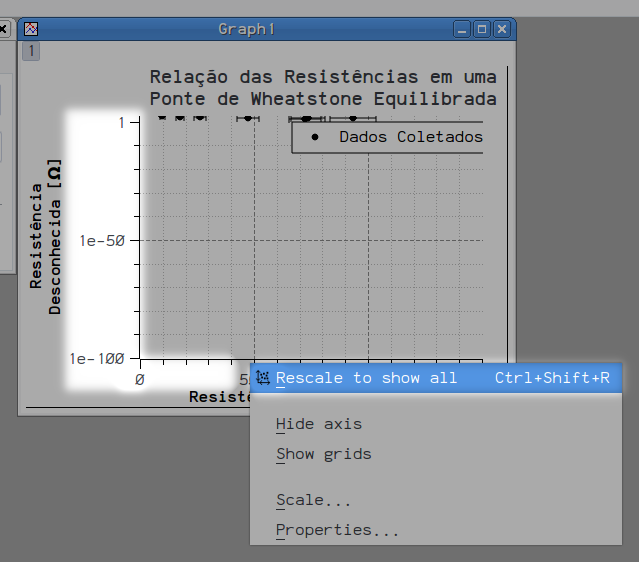
\includegraphics[width=\textwidth]{escala/2rescale.png}

            \caption{Mudança automática dos limites do gráfico}
            \label{fig:escala:rescale}
        \end{subfigure}
        ~
        \begin{subfigure}{0.45\textwidth}
            \centering
            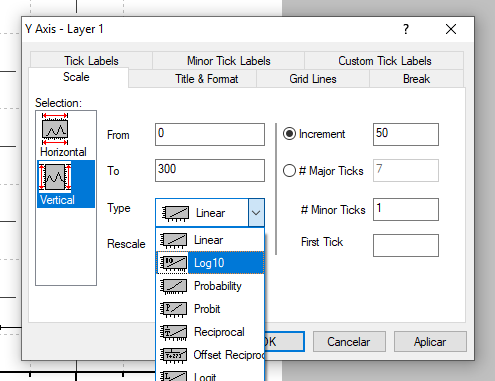
\includegraphics[width=\textwidth]{escala/3logscale.png}

            \caption{Escala logarítmica de base 10}
            \label{fig:escala:logscale}
        \end{subfigure}
        \caption{Colocando a escala logarítmica}
        \label{fig:escala:tutorial}
    \end{figure}

    \begin{figure}[htbp]
        \centering
        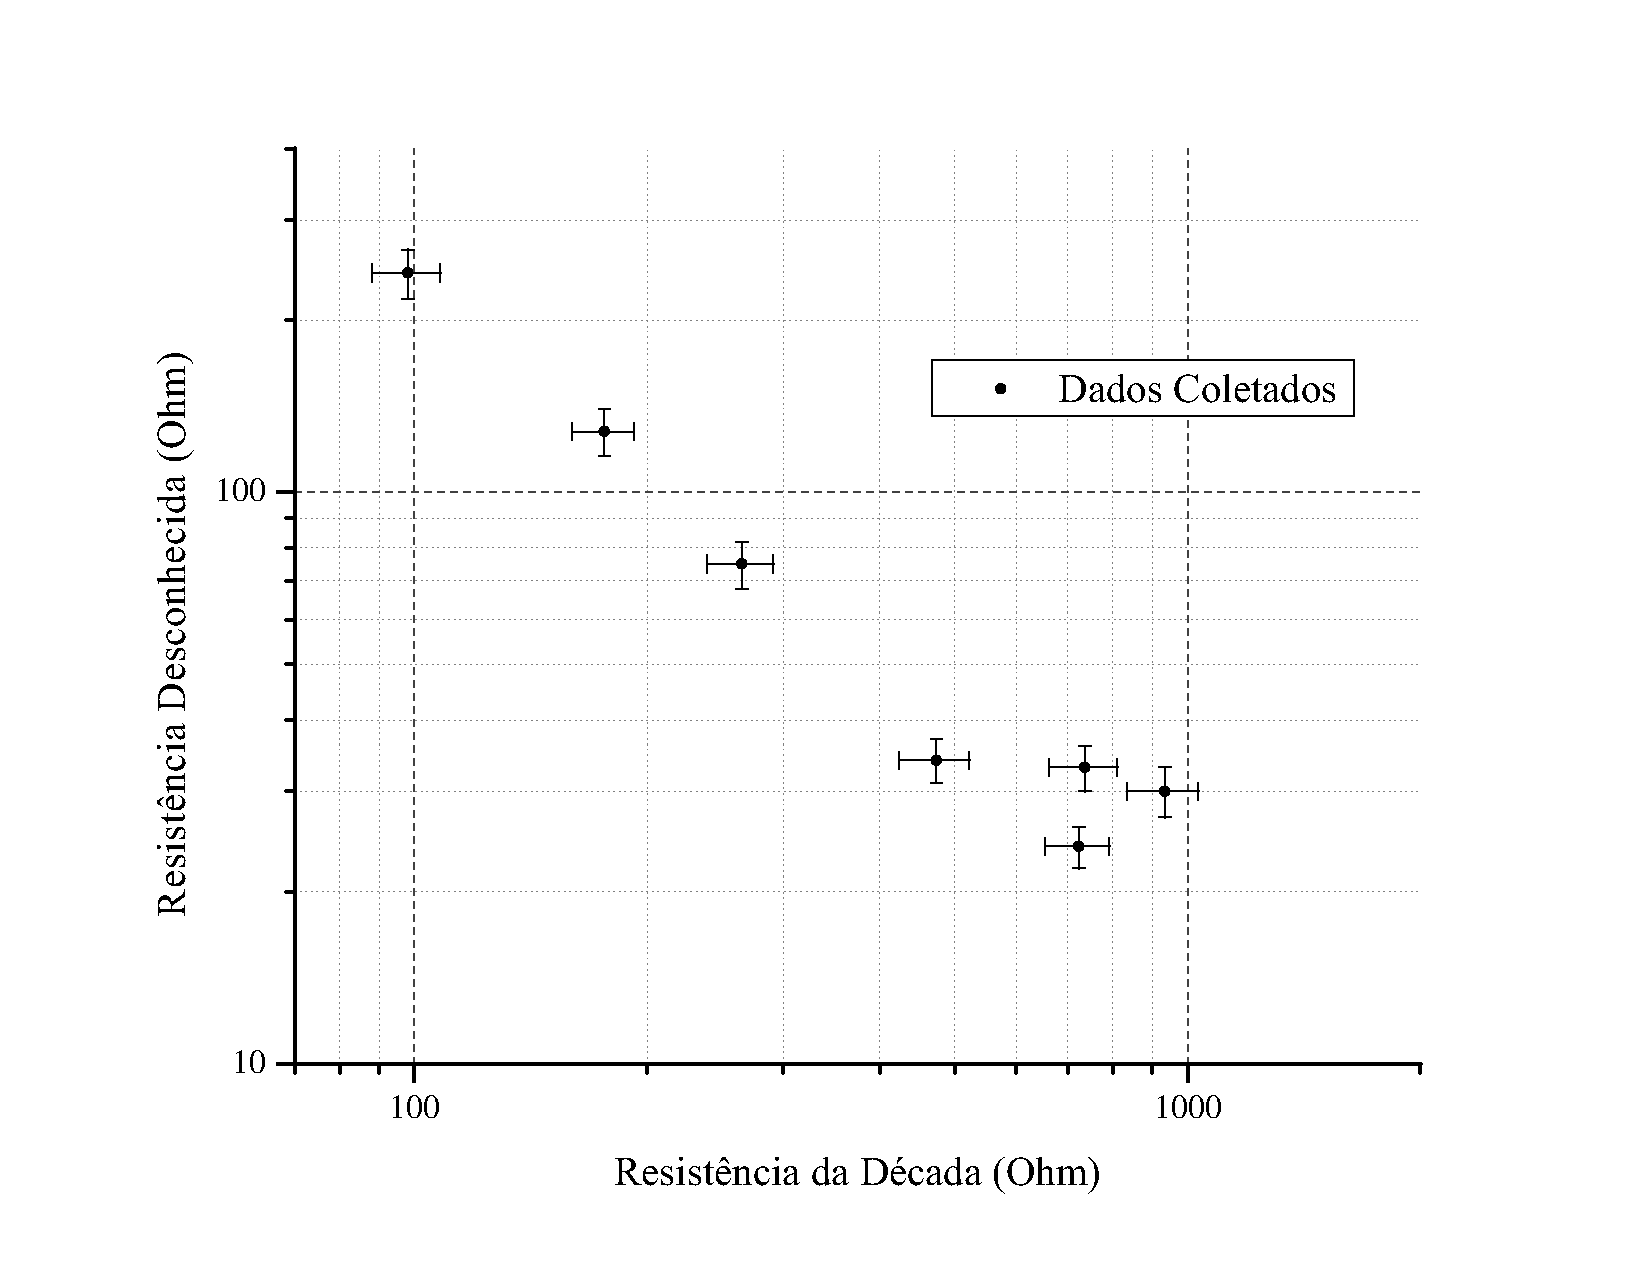
\includegraphics[width=0.8\textwidth]{escala/4loglog.pdf}

        \caption{Gráfico \texttt{log-log} dos dados da figura \ref{fig:escala:loglog:dados}}
        \label{fig:escala:loglog:resultado}
    \end{figure}


\subsection{Gráfico Semi-Log}

    \begin{figure}[htbp]
        \centering
        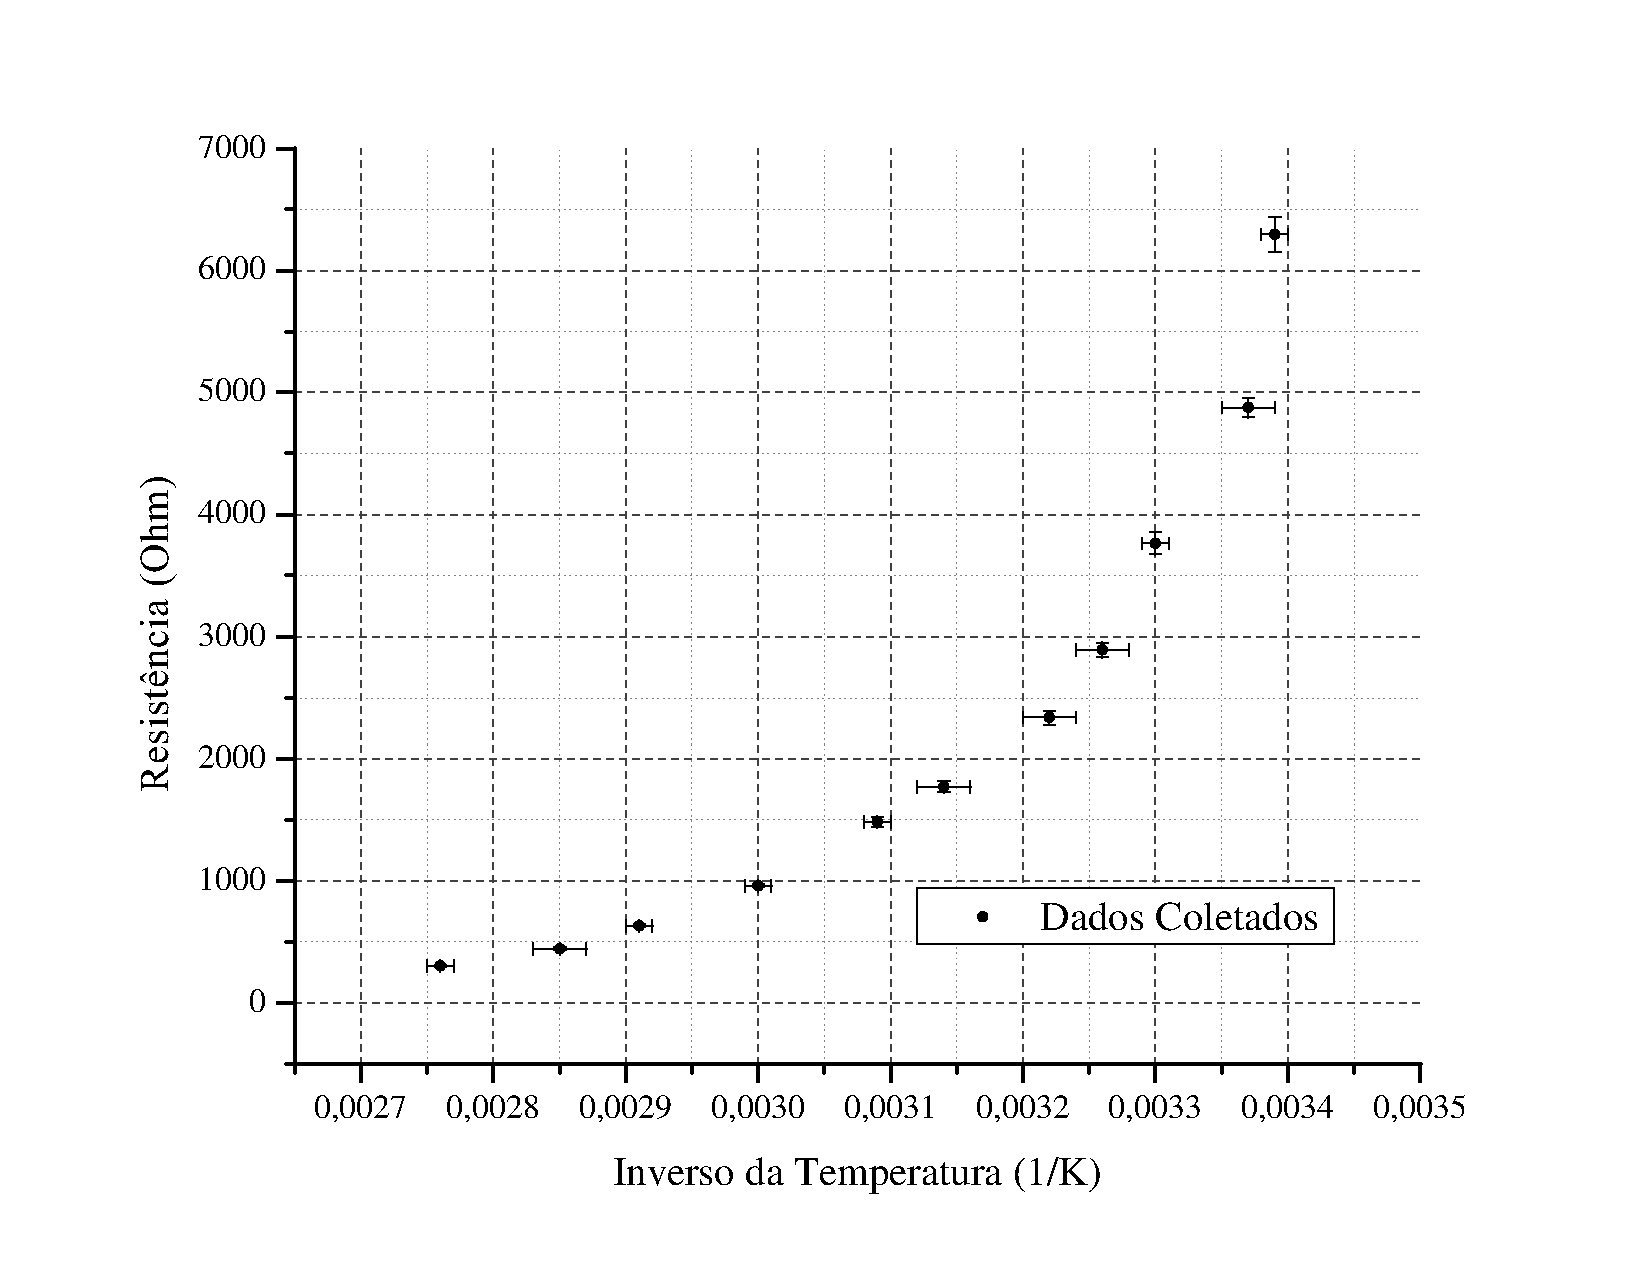
\includegraphics[width=0.6\textwidth]{escala/5dados.pdf}

        \caption{Gráfico da relação (\ref{eq:termistor}) do termistor}
        \label{fig:escala:semilog:dados}
    \end{figure}

    \begin{equacao} \label{eq:termistor}
        R = A ~ \exp\left(B ~ T^{-1}\right)
    \end{equacao}

    Agora com os dados da figura \ref{fig:escala:semilog:dados} e a relação (\ref{eq:termistor}), com $R$ como a resistência e $T^{-1}$ o inverso da temperatura, a linearização se torna:

    \begin{align*}
        \ln(R)
            &= \ln\left(A ~ \exp\left(B ~ T^{-1}\right) \right) \\
            &= \ln(A) + \ln\left(\exp\left(B ~ T^{-1}\right) \right) \\
            &= \ln(A) + B ~ T^{-1}
    \end{align*}

    Que pode ser usada em um gráfico \texttt{semi-log} de $R \times T^{-1}$, como na figura \ref{fig:escala:tutextra}.

    \begin{figure}[htbp]
        \centering
        \begin{subfigure}{0.45\textwidth}
            \centering
            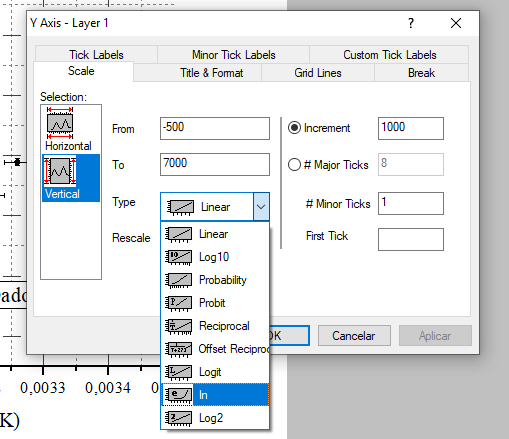
\includegraphics[width=\textwidth]{escala/6lnscale.png}

            \caption{Escala logarítmica de base $e$}
            \label{fig:escala:lnscale}
        \end{subfigure}
        ~
        \begin{subfigure}{0.45\textwidth}
            \centering
            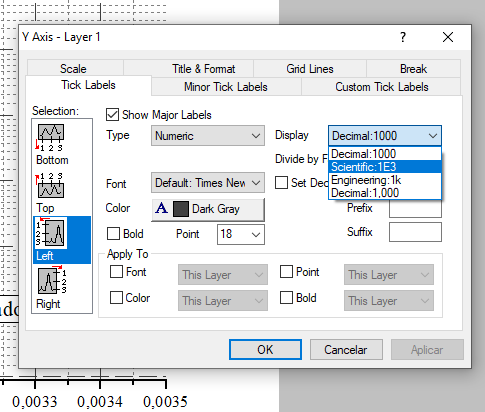
\includegraphics[width=\textwidth]{escala/7expticks.png}

            \caption{Marcadores de escala como expoentes de $e$}
            \label{fig:escala:expticks}
        \end{subfigure}
        \caption{Ajustes para a escala \texttt{ln}}
        \label{fig:escala:tutextra}
    \end{figure}

    \begin{figure}[htbp]
        \centering
        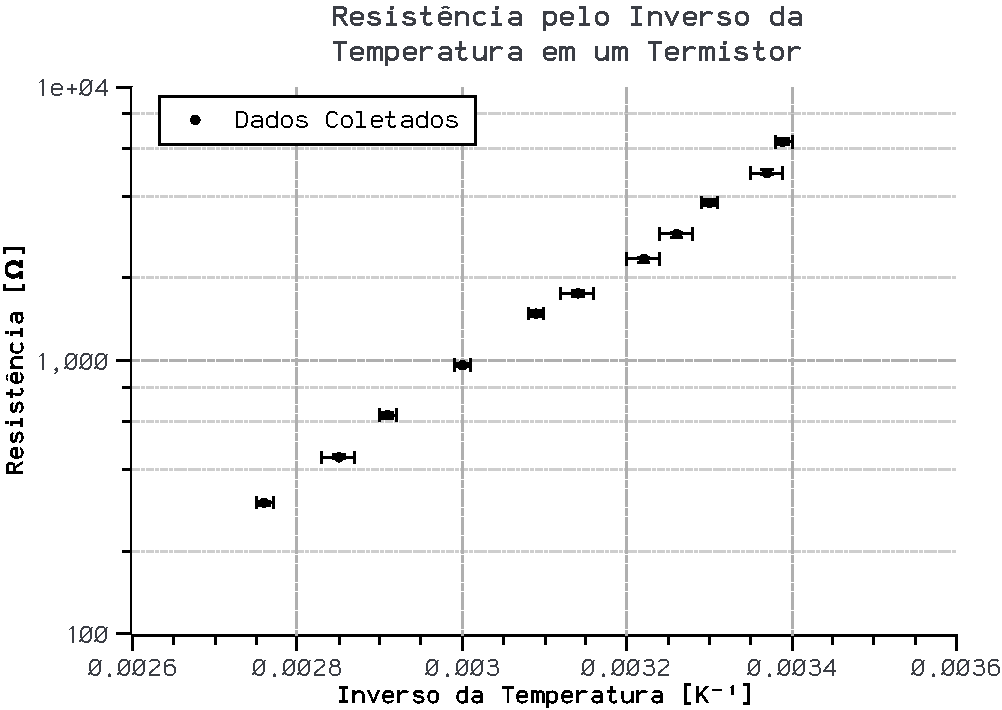
\includegraphics[width=0.8\textwidth]{escala/8semilog.pdf}

        \caption{Gráfico \texttt{semi-log} dos dados da figura \ref{fig:escala:semilog:dados}}
        \label{fig:escala:semilog:resultado}
    \end{figure}


\subsection{Regressão em Escala Logarítmica}

    A regressão de uma curva de potência ou exponencial é possível com técnicas de regressão não-linear, só que essas técnicas não cabem no escopo dessa matéria. Uma outra opção muito utilizada é encontrar uma linearização, como na equação (\ref{eq:linearizacao}), e, com a nova relação linear de $f(x, y) \times g(x, y)$, aplicar a regressão linear como da seção \nameref{sec:regres}. O único detalhe é que é preciso encontrar os valores de $f(x, y)$ e $g(x, y)$ e suas incertezas para cada par $(x, y)$ dos dados e só com esses valores pode-se encontrar os coeficientes $a$ e $b$, como foi feito na figura \ref{fig:escala:regres}.

    \begin{figure}[htbp]
        \centering
        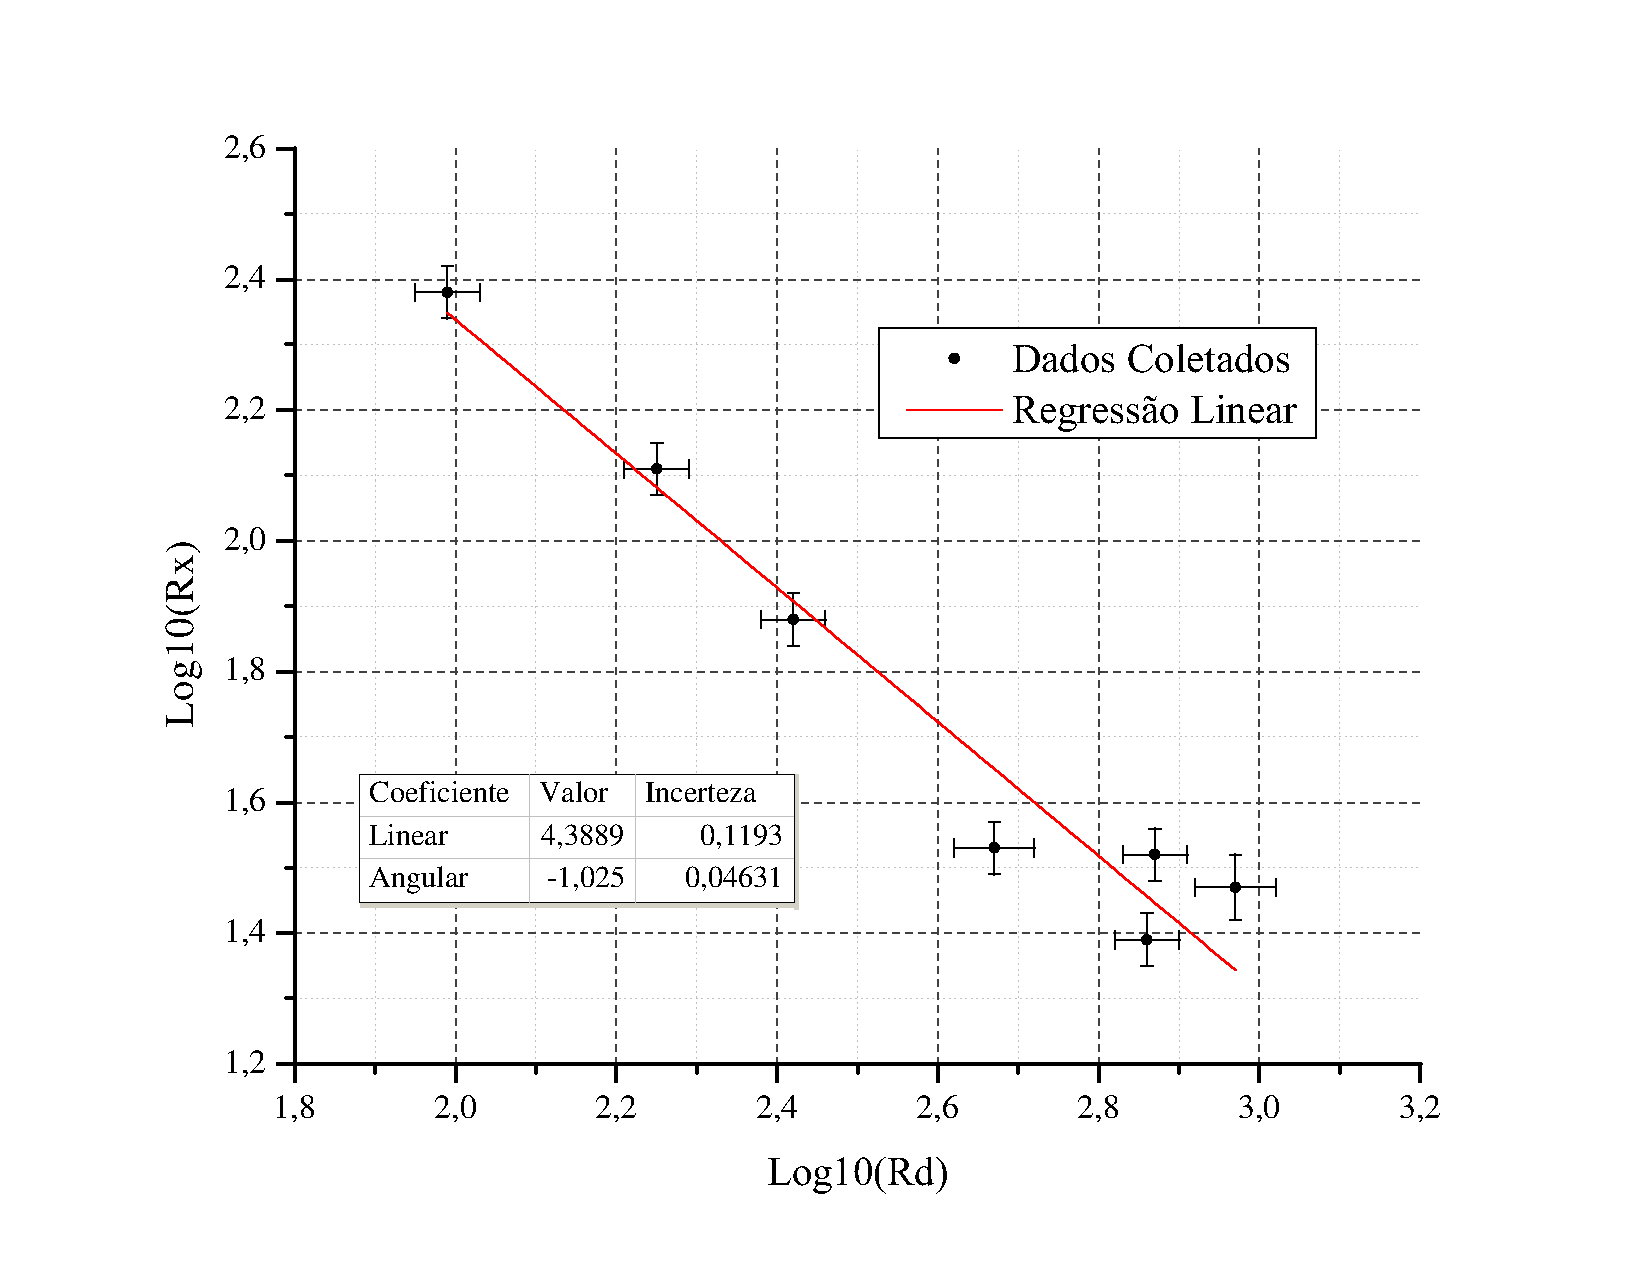
\includegraphics[width=0.8\textwidth]{escala/9logreg.pdf}

        \caption{Gráfico da regressão da relação (\ref{eq:wheatstone}). Isso seviria para mostrar que $b \approx -1$, por exemplo.}
        \label{fig:escala:regres}
    \end{figure}

    A mudança dos dados de $(x, y)$ para $(f(x, y), g(x, y))$ ajuda nos cálculos, só que normalmente causa um distanciamento do sentido físco dos dados. Então, é importante decidir qual dos gráficos utilizar ou se cabe usar os dois gráficos.


    \section{Equação Característica} \label{sec:caract}
        % Um exemplo de equação característica é a equação (\ref{eq:termistor}), do termistor, que será utilizada nesta seção. Os dados gerados para o gráfico \ref{fig:escala:semilog:dados} continuarão os mesmos aqui.

\subsection{Encontrando os Coeficientes}

    O primeiro passo normalmente é encontrar os coeficientes da equação característica. Se for uma equação de reta, uma simples regressão linear é bastante para encontrar esses coeficientes e para mostrar a equação esperada.

    Para os outros caso, no entanto, é preciso linearizar a equação, como feito na seção \nameref{sec:escala}, encontrar os coeficientes da linearização e transformar para os coeficientes da equação inicial.

    No caso dos dados do termistor, a regressão é aplicada como na figura \ref{fig:caract:regres}. Logo, os coeficientes se tornam $A = \exp(-7.095) \approxeq 0.0008293$ e $B = 4643.029$.

    \begin{figure}[htbp]
        \centering
        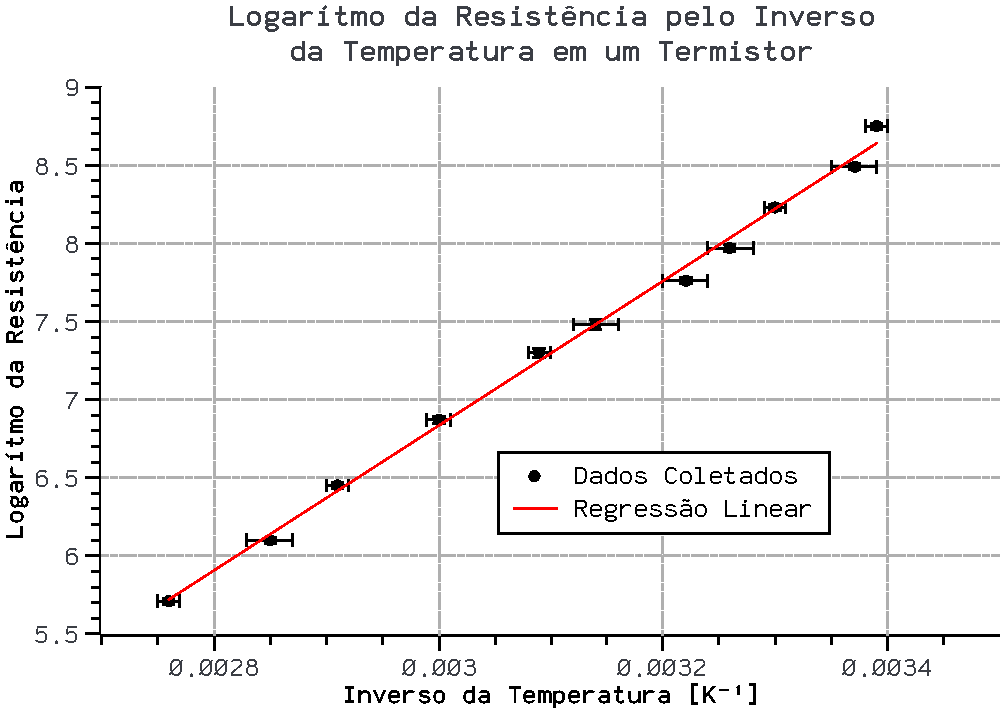
\includegraphics[width=0.6\textwidth]{caract/1regres.pdf}

        \caption{Gráfico da linearização da equação (\ref{eq:termistor})}
        \label{fig:caract:regres}
    \end{figure}


    \subsection{Gráfico de Funções}

    Voltando para os dados originais, de $R$ por $T$, podemos desenhar a equação característica, agora com os valores dos coeficientes, sobre o \texttt{Scatter} dos dados, como mostra a figura \ref{fig:caract:inserir}.

    \begin{figure}[htbp]
        \centering
        \begin{subfigure}{0.4\textwidth}
            \centering
            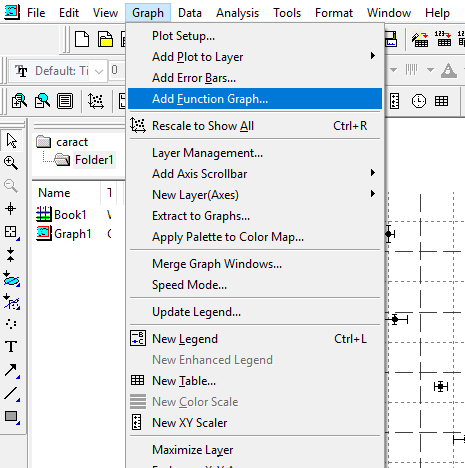
\includegraphics[width=\textwidth]{caract/2insert.png}

            \caption{Adicionando uma função no gráfico}
            \label{fig:caract:novo}
        \end{subfigure}
        ~
        \begin{subfigure}{0.55\textwidth}
            \centering
            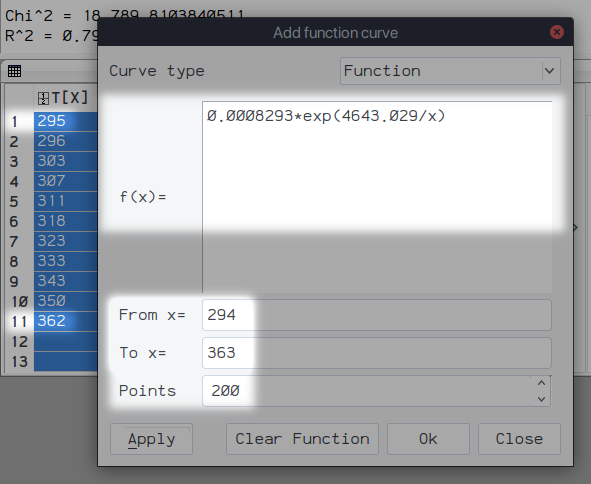
\includegraphics[width=\textwidth]{caract/4funcao.png}

            \caption{Colocando a função $R = 0.0008293 ~ \exp(4643.029/T)$}
            \label{fig:caract:funcao}
        \end{subfigure}
        \caption{Desenhando uma função no gráfico}
        \label{fig:caract:inserir}
    \end{figure}


\subsection{Ajustes de Formatação}

    Por padrão, a cor da nova curva do gráfico é escolhida como preto, mas isso pode ser mudado com um duplo clique sobre a curva. Neste exemplo a cor decidida foi vermelho, que acompanha o padrão de regressão dos exemplos anteriores.

    \begin{figure}[htbp]
        \centering
        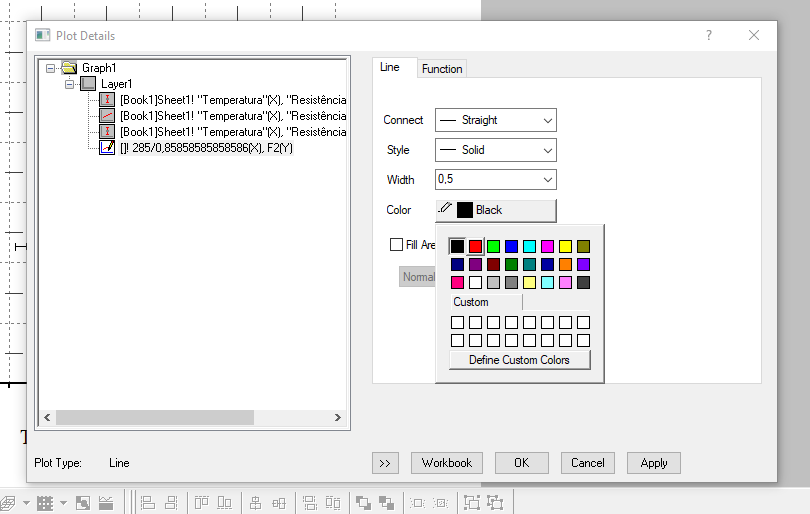
\includegraphics[width=0.8\textwidth]{caract/5cor.png}

        \caption{Mudança da cor da nova curva}
        \label{fig:caract:cor}
    \end{figure}

    Além da cor, é importante lembrar de tratar da curva na legenda do gráfico. Para isso, basta escolher uma legenda mais descritiva para a curva.

\subsection{Resultado}

    \begin{figure}[htbp]
        \centering
        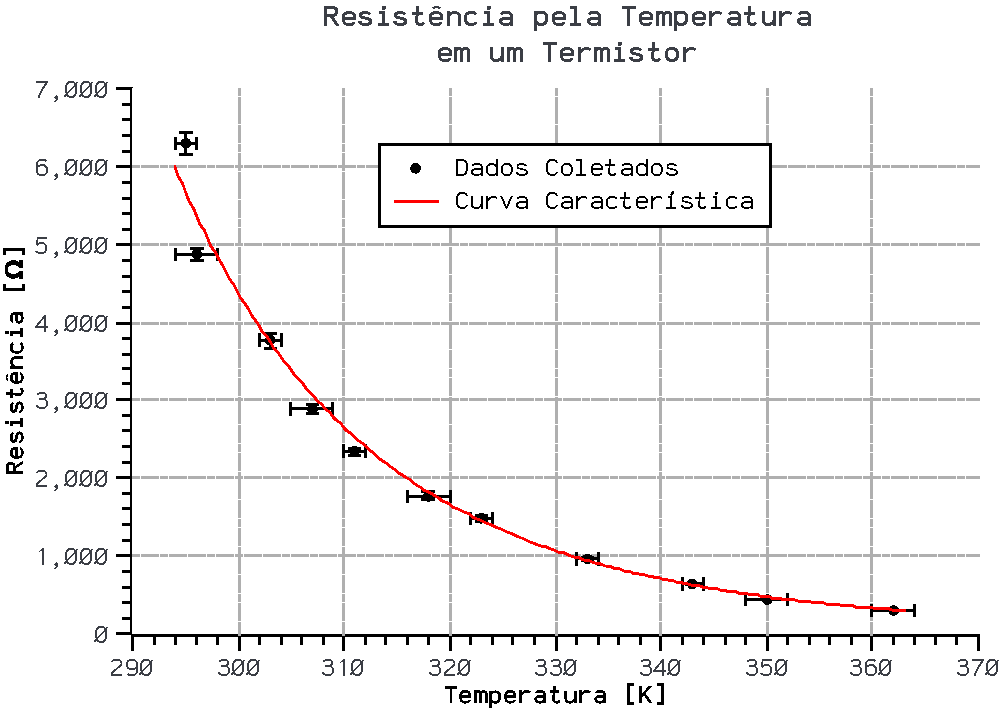
\includegraphics[width=0.6\textwidth]{caract/8final.pdf}

        \caption{Gráfico com a curva característica do termistor}
        \label{fig:caract:final}
    \end{figure}


    \section{Gráficos de Múltiplas Variáveis} \label{sec:multiv}
        % \edef\indentacao{\the\parindent}

\noindent
\begin{minipage}[t]{0.55\textwidth}\setlength{\parindent}{\indentacao}

    Para os casos em que é necessário apresentar dados com mais de uma váriavel dependente de um mesmo dado \texttt{X}, existe a opção de gráficos múltiplos. Eles servem para comparar as relações do tipo $y_1 = f(x)$ e $y_2 = g(x)$, quando $x$, $y_1$ e $y_2$ são medidos em conjunto.

    Em experimentos com circuitos, esse tipo de dado aparece, por exemplo, na medição de tensão em nós diferentes para a comparação de seus comportamentos no tempo. É o caso do circuito da figura \ref{fig:multiv:circuito}, cujos dados foram colocados como na figura \ref{fig:multiv:dados}.

    \begin{figure}[H]
        \centering
        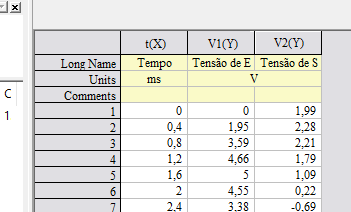
\includegraphics[width=0.8\textwidth]{multiv/1dados.png}

        \caption{Dados gerados com simulador}
        \label{fig:multiv:dados}
    \end{figure}

\end{minipage}\vspace{0.05\textwidth}%
\begin{minipage}[t]{0.4\textwidth}
    \begin{figure}[H]
        \centering
        \begin{circuitikz}[scale=1.2]

    \draw (2, 0)
    to [short] ++(-2,0)
    to [vsourcesin, l=$E$] ++(0,4)
    to [short] ++(2,0)
    to [resistor, l_=$R$] ++(0,-2)
    to [capacitor, l_=$C$] ++(0,-2)
    node[ground] {};

    \draw [->, thick] (3,4) to node[above] {$V_1$} (2.1,4);

    \draw [->, thick] (3,2) to node[above] {$V_2$} (2.1,2);

\end{circuitikz}


        \caption{Circuito de defasagem da tensão por um capacitor}
        \label{fig:multiv:circuito}
    \end{figure}
\end{minipage}


\subsection{Gráficos de Eixos Separados}

    Uma opção para mostrar os dois canais ao mesmo tempo é colocar cada um em seu próprio gŕafico com seus próprios eixos. No \texttt{Origin}, isso é feito como na figura \ref{fig:multiv:paneis:tutorial}, mas pode ser feito em duas imagens separadas também. O problema com essa abordagem é que as escalas diferentes não mostram muito bem as proporções entre os canais de entrada e saída.

    \begin{figure}[H]
        \centering
        \includegraphics[width=0.6\textwidth]{multiv/2paneis.png}

        \caption{Criando os gráficos separados}
        \label{fig:multiv:paneis:tutorial}
    \end{figure}

    \begin{figure}[H]
        \centering
        \includegraphics[width=0.8\textwidth]{multiv/3paneis.pdf}

        \caption{Gráficos das tensões de entrada e saída do circuito}
        \label{fig:multiv:paneis}
    \end{figure}


\subsection{Gráficos de Eixos em Conjunto}

    \begin{figure}[htbp]
        \centering
        \includegraphics[width=0.6\textwidth]{multiv/4dois.png}

        \caption{Criando o gráfico com as duas curvas}
        \label{fig:multiv:juntos:tutorial}
    \end{figure}

    \noindent
    \begin{minipage}[t]{0.35\textwidth}
        \begin{figure}[H]
            \centering
            \includegraphics[width=\textwidth]{multiv/5dois.png}

            \caption{Formatação do rótulo dos eixos}
            \label{fig:multiv:juntos:formatacao}
        \end{figure}
    \end{minipage}\hspace{0.05\textwidth}%
    \begin{minipage}[t]{0.6\textwidth}\setlength{\parindent}{\indentacao}

        Quando o gráfico é criado como na figura \ref{fig:multiv:juntos:tutorial}, o que rótulo do eixo $y$ fica como o nome de apenas uma das colunas dos dados. Pra consertar isso basta alterar o nome do eixo para algum texto que descreve ambas variáveis (figura \ref{fig:multiv:juntos:formatacao}).

        Um dos maiores limites para esse método é que as variáveis dependentes precisam ter a mesma motivação física e, por causa disso, a mesma gradeza, caso contrário, o eixo compartilhado entre elas perde completamente o sentido.

    \end{minipage}

    \begin{figure}[htbp]
        \centering
        \includegraphics[width=0.8\textwidth]{multiv/6dois.pdf}

        \caption{Gráfico das tensões $V_1$ e $V_2$ do circuito}
        \label{fig:multiv:juntos}
    \end{figure}


\subsection{Gráficos com Apenas a Abscissa Comum}

    \begin{figure}[htbp]
        \centering
        \includegraphics[width=0.6\textwidth]{multiv/7duplo.png}

        \caption{Criando o gráfico com três eixos}
        \label{fig:multiv:duplo:tutorial}
    \end{figure}

    Imagine agora o caso em que queremos mostrar a defasagem entre a corrente a tensão no capacitor da figura \ref{fig:multiv:circuito}. A única grandeza comum agora é o tempo, então vamos precisar de gráficos de três eixos. No \texttt{Origin}, isso é feito como mostra a imagem \ref{fig:multiv:duplo:tutorial}. Normalmente, é melhor alterar as cores para melhor representar cada dado.

    \begin{figure}[htbp]
        \centering
        \includegraphics[width=0.8\textwidth]{multiv/8duplo.pdf}

        \caption{Gráfico de corrente e tensão em um capacitor por tempo}
        \label{fig:multiv:duplo}
    \end{figure}

    \begin{nota}
        As vezes, os gráficos com múltiplas curvas podem ficar sobrecarregado de informação. Quando isso acontece, o melhor é separar os dados em gráficos distintos pra manter a legibilidade. Gráficos de três eixos pdem ficar complicados com facilidade.
    \end{nota}


    \section{Curvas de Nível} \label{sec:contorno}
    %     Curvas de nível servem para representar dados tridimensionais em um plano. As três variáveis para esse tipo de gráfico são $x$ e $y$ independentes e $z = f(x,y)$.

Serão usados, como exemplo, dados semelhantes aos do experimento sobre potencial elétrico entre barras de cobre em uma solução condutiva. Nesse caso, as variáveis dependentes são as distâncias $x$ e $y$ no plano e a variável dependente é o potencial $V$ de cada ponto.


\subsection{Limitações do SciDavis}

    Com o \software, as opções para fazer curvas de nível são bem mais limitadas do que com outras ferramentas e os resultados costumam ter muitos problemas de formatação. Observe na figura \ref{fig:contorno:limitado} como é difícil a leitura dos níveis com as cores e como os níveis não fazem muito sentido. Além disso, esse modelo de gráfico serve apenas para pontos igualmente espaçados de $x$ e $y$.

    \begin{figure}[htbp]
        \centering
        \includegraphics[width=0.6\textwidth]{contorno/limitado.png}

        \caption{Exemplos de gráfico de curvas de nível do \software}
        \label{fig:contorno:limitado}
    \end{figure}


\subsection{Simulando Curvas de Nível}

    Apesar de tudo isso, é possível simular curvas de nível com um gráfico de múltiplas variáveis. Para tanto, é preciso que os dados sejam coletados seguindo valores fixos de $x$ e,$z$ que significa medir as equipotenciais em valores específicos de $x$ no caso das medidas de potencial na cuba.

    \begin{figure}[htbp]
        \centering
        \includegraphics[width=0.6\textwidth]{contorno/1dados.png}

        \caption{Montagem dos dados de posições para cada potencial}
        \label{fig:contorno:dados}
    \end{figure}

    No \software, basta separar os valores de cada $z$ diferente em colunas próprias de $y$. A tabela deve ficar algo parecido com a da figura \ref{fig:contorno:dados}. Com isso, basta aplicar o mesmo processo de montagem do gráficoda seção \nameref{sec:multiv:juntos}.


\subsection{Opções de Formatação}

    Por padrão, o \software coloca cores variadas para cada nível, mas é mais recomendado seguir tons variados de uma mesma cor. Para este exemplo será seguido um padrão de cores monocromáticas. Além disso, a grossura das linhas (\texttt{Line width}) foi alterada para o valor 2.

    \begin{figure}[htbp]
        \centering
        \includegraphics[width=0.6\textwidth]{contorno/2cor.png}

        \caption{Principais opções de formatação}
        \label{fig:contorno:cor}
    \end{figure}

    \begin{lembrete}
        É importante a adição de sufixos com a unidade do valor medido na legenda.
    \end{lembrete}


\subsection{Resultado}

    \begin{figure}[htbp]
        \centering
        \includegraphics[width=0.6\textwidth]{contorno/resultado.pdf}

        \caption{Deformação das equipotenciais gerada pela adição de uma ponta}
        \label{fig:contorno:final}
    \end{figure}



\end{document}
